%%%%%%%%%%%%%%%%%%%%%%%%%%%%%%%%%%%%%%%%%
% Masters/Doctoral Thesis 
% LaTeX Template
% Version 2.5 (27/8/17)
%
% This template was downloaded from:
% http://www.LaTeXTemplates.com
%
% Version 2.x major modifications by:
% Vel (vel@latextemplates.com)
%
% This template is based on a template by:
% Steve Gunn (http://users.ecs.soton.ac.uk/srg/softwaretools/document/templates/)
% Sunil Patel (http://www.sunilpatel.co.uk/thesis-template/)
%
% Template license:
% CC BY-NC-SA 3.0 (http://creativecommons.org/licenses/by-nc-sa/3.0/)
%
%%%%%%%%%%%%%%%%%%%%%%%%%%%%%%%%%%%%%%%%%

%----------------------------------------------------------------------------------------
%	PACKAGES AND OTHER DOCUMENT CONFIGURATIONS
%----------------------------------------------------------------------------------------

\documentclass[
11pt, % The default document font size, options: 10pt, 11pt, 12pt
oneside, % Two side (alternating margins) for binding by default, uncomment to switch to one side
english, % ngerman for German
singlespacing, % Single line spacing, alternatives: onehalfspacing or doublespacing
%draft, % Uncomment to enable draft mode (no pictures, no links, overfull hboxes indicated)
%nolistspacing, % If the document is onehalfspacing or doublespacing, uncomment this to set spacing in lists to single
%liststotoc, % Uncomment to add the list of figures/tables/etc to the table of contents
%toctotoc, % Uncomment to add the main table of contents to the table of contents
parskip, % Uncomment to add space between paragraphs
%nohyperref, % Uncomment to not load the hyperref package
headsepline, % Uncomment to get a line under the header
%chapterinoneline, % Uncomment to place the chapter title next to the number on one line
consistentlayout, % Uncomment to change the layout of the declaration, abstract and acknowledgements pages to match the default layout
]{MastersDoctoralThesis} % The class file specifying the document structure

\usepackage[utf8]{inputenc} % Required for inputting international characters
\usepackage[T1]{fontenc} % Output font encoding for international characters

\usepackage{mathpazo} % Use the Palatino font by default
\usepackage{csvsimple}
\usepackage{booktabs}
\usepackage{amsmath}
\usepackage{graphicx}
\usepackage{longtable}
\usepackage{array}
\usepackage{lscape}
\usepackage{adjustbox}
\usepackage{siunitx}
\usepackage{pdflscape}
\usepackage[backend=bibtex,style=numeric,sorting=none,natbib=true]{biblatex} % Use the bibtex backend with the authoryear citation style (which resembles APA)

\addbibresource{example.bib} % The filename of the bibliography

\usepackage[autostyle=true]{csquotes} % Required to generate language-dependent quotes in the bibliography
%----------------------------------------------------------------------------------------
%	MARGIN SETTINGS
%----------------------------------------------------------------------------------------

\geometry{
	paper=a4paper, % Change to letterpaper for US letter
	inner=2.5cm, % Inner margin
	outer=3.8cm, % Outer margin
	bindingoffset=.5cm, % Binding offset
	top=1.5cm, % Top margin
	bottom=1.5cm, % Bottom margin
	%showframe, % Uncomment to show how the type block is set on the page
}

%----------------------------------------------------------------------------------------
%	THESIS INFORMATION
%----------------------------------------------------------------------------------------

\thesistitle{Microelectronic circuit design for neural interfaces in 0.13µm CMOS technology using an open source VLSI ecosystem} % Your thesis title, this is used in the title and abstract, print it elsewhere with \ttitle
\supervisor{Prof. Andreas \textsc{Hierlemann}
			\\ Dr. Fernando \textsc{Cardes}} % Your supervisor's name, this is used in the title page, print it elsewhere with \supname
\examiner{} % Your examiner's name, this is not currently used anywhere in the template, print it elsewhere with \examname
\degree{Master in Electrical Engineering} % Your degree name, this is used in the title page and abstract, print it elsewhere with \degreename
\author{Rafael Miguel \textsc{Correa}} % Your name, this is used in the title page and abstract, print it elsewhere with \authorname
\addresses{} % Your address, this is not currently used anywhere in the template, print it elsewhere with \addressname

\subject{Electrical Engineering} % Your subject area, this is not currently used anywhere in the template, print it elsewhere with \subjectname
\keywords{} % Keywords for your thesis, this is not currently used anywhere in the template, print it elsewhere with \keywordnames
\university{\href{https://ethz.ch/en.html}{ETHZ}} % Your university's name and URL, this is used in the title page and abstract, print it elsewhere with \univname
\department{\href{http://department.university.com}{D-ITET}} % Your department's name and URL, this is used in the title page and abstract, print it elsewhere with \deptname
\group{\href{http://researchgroup.university.com}{BEL}} % Your research group's name and URL, this is used in the title page, print it elsewhere with \groupname
\faculty{\href{https://ee.ethz.ch}{D-ITET}} % Your faculty's name and URL, this is used in the title page and abstract, print it elsewhere with \facname

\AtBeginDocument{
\hypersetup{pdftitle=\ttitle} % Set the PDF's title to your title
\hypersetup{pdfauthor=\authorname} % Set the PDF's author to your name
\hypersetup{pdfkeywords=\keywordnames} % Set the PDF's keywords to your keywords
}

\begin{document}

\hypersetup{
    colorlinks=false,  % Enable colored links
    linkcolor=red,  % Color for internal links (e.g., sections, pages)
    citecolor=red,  % Color for citations
    urlcolor=red   % Color for URLs
}

\frontmatter % Use roman page numbering style (i, ii, iii, iv...) for the pre-content pages

\pagestyle{plain} % Default to the plain heading style until the thesis style is called for the body content

%----------------------------------------------------------------------------------------
%	TITLE PAGE
%----------------------------------------------------------------------------------------

\begin{titlepage}
\begin{center}

\vspace*{.06\textheight}
{\scshape\LARGE \univname\par}\vspace{1.5cm} % University name
\textsc{\Large Semester Project Report}\\[0.5cm] % Thesis type

\HRule \\[0.4cm] % Horizontal line
{\huge \bfseries \ttitle\par}\vspace{0.4cm} % Thesis title
\HRule \\[1.5cm] % Horizontal line
 
\begin{minipage}[t]{0.4\textwidth}
\begin{flushleft} \large
\emph{Author:}\\
{\authorname} % Author name - remove the \href bracket to remove the link
\end{flushleft}
\end{minipage}
\begin{minipage}[t]{0.4\textwidth}
\begin{flushright} \large
\emph{Supervisor:} \\
{\supname} % Supervisor name - remove the \href bracket to remove the link  
\end{flushright}
\end{minipage}\\[3cm]
 
\vfill

\large \textit{\degreename}\\[0.3cm] % University requirement text
\textit{}\\[0.4cm]
\deptname\\[2cm] % Research group name and department name
 
\vfill

{\large \today}\\[4cm] % Date
%\includegraphics[h!][width=0.2\textwidth]{Figures/ETHZ.png} % University/department logo - uncomment to place it
 
\vfill
\end{center}
\end{titlepage}

%----------------------------------------------------------------------------------------
%	DECLARATION PAGE
%----------------------------------------------------------------------------------------

% \begin{declaration}
% \addchaptertocentry{\authorshipname} % Add the declaration to the table of contents
% \noindent I, \authorname, declare that this thesis titled, \enquote{\ttitle} and the work presented in it are my own. I confirm that:

% \begin{itemize} 
% \item This work was done wholly or mainly while in candidature for a research degree at this University.
% \item Where any part of this thesis has previously been submitted for a degree or any other qualification at this University or any other institution, this has been clearly stated.
% \item Where I have consulted the published work of others, this is always clearly attributed.
% \item Where I have quoted from the work of others, the source is always given. With the exception of such quotations, this thesis is entirely my own work.
% \item I have acknowledged all main sources of help.
% \item Where the thesis is based on work done by myself jointly with others, I have made clear exactly what was done by others and what I have contributed myself.\\
% \end{itemize}
 
% \noindent Signed:\\
% \rule[0.5em]{25em}{0.5pt} % This prints a line for the signature
 
% \noindent Date:\\
% \rule[0.5em]{25em}{0.5pt} % This prints a line to write the date
% \end{declaration}

% \cleardoublepage

%----------------------------------------------------------------------------------------
%	QUOTATION PAGE
%----------------------------------------------------------------------------------------

% \vspace*{0.2\textheight}

% \noindent\enquote{\itshape Thanks to my solid academic training, today I can write hundreds of words on virtually any topic without possessing a shred of information, which is how I got a good job in journalism.}\bigbreak

% \hfill Dave Barry

%----------------------------------------------------------------------------------------
%	ABSTRACT PAGE
%----------------------------------------------------------------------------------------

\begin{abstract}
\addchaptertocentry{\abstractname} % Add the abstract to the table of contents
This semester project, titled "Microelectronic Circuit Design for Neural Interfaces in 0.13µm CMOS Technology Using an Open Source VLSI Ecosystem," explores the capabilities of IC design using open-source tools by developing a CMOS inverter-based amplifier for neural interfaces.

The primary objectives are to develop a CMOS inverter-based amplifier that meets specific design specifications, demonstrate the capabilities of various open-source tools throughout the IC design workflow, and create a comprehensive guide for future projects within the BEL group. The design workflow utilizes tools such as Xschem for schematic capture, Ngspice for circuit simulation, Magic for layout design, and Netgen for layout versus schematic (LVS) checks, all integrated with the SkyWater SKY130 PDK.

The designed amplifier aims to provide effective amplification with good signal-to-noise ratio (SNR), low noise, and low power consumption, which is crucial for high-fidelity neural recordings. This project highlights the potential of open-source tools to reduce development costs and foster collaboration within the BEL group.

By the conclusion of this project, a robust CMOS inverter-based amplifier design was successfully simulated and verified, making it ready for fabrication. The extensive documentation provided serves as a valuable reference for future open-source IC design projects within the BEL group, significantly contributing to the group's knowledge base and technical capabilities.
\end{abstract}

%----------------------------------------------------------------------------------------
%	ACKNOWLEDGEMENTS
%----------------------------------------------------------------------------------------

\begin{acknowledgements}
\addchaptertocentry{\acknowledgementname} % Add the acknowledgements to the table of contents
I would like to extend my gratitude to Prof. Dr. Andreas Hierlemann for enabling this project.

My deepest thanks go to Dr. Fernando Cardes, who was instrumental throughout the entire project. His extensive support, guidance, and responsiveness were crucial to my work. Working with him has been an exceptionally experience, and I am thankful for his dedication.

Additionally, I appreciate Prof. Dr. Hanspeter Schmid for his help with the circuit analysis using the Driving Point Signal Flow Graph (DPSFG) method, which was vital for determining the transfer function.

In preparing my report, I sought assistance from ChatGPT (\textcite{chatgpt}) to help reformulate and improve the clarity of certain sections of my report.
\end{acknowledgements}

%----------------------------------------------------------------------------------------
%	LIST OF CONTENTS/FIGURES/TABLES PAGES
%----------------------------------------------------------------------------------------

\setcounter{tocdepth}{1}
\tableofcontents % Prints the main table of contents

\listoffigures % Prints the list of figures

\listoftables % Prints the list of tables

%----------------------------------------------------------------------------------------
%	ABBREVIATIONS
%----------------------------------------------------------------------------------------


\begin{abbreviations}{ll} % Include a list of abbreviations (a table of two columns)
	\textbf{AC} & \textbf{A}lternating \textbf{C}urrent \\
	\textbf{APS} & \textbf{A}ctive \textbf{P}ixel \textbf{S}ensor \\
	\textbf{BEL} & \textbf{B}io\textbf{s}ystems \textbf{S}cience and \textbf{E}ngineering \\
	\textbf{CMOS} & \textbf{C}omplementary \textbf{M}etal-\textbf{O}xide-\textbf{S}emiconductor \\
	\textbf{DC} & \textbf{D}irect \textbf{C}urrent \\
	\textbf{DRC} & \textbf{D}esign \textbf{R}ule \textbf{C}heck \\
    \textbf{DPSFG} & \textbf{D}riving \textbf{P}oint \textbf{S}ignal \textbf{F}low \textbf{G}raph \\
	\textbf{IC} & \textbf{I}ntegrated \textbf{C}ircuit \\
	\textbf{LVS} & \textbf{L}ayout \textbf{V}ersus \textbf{S}chematic \\
	\textbf{PDK} & \textbf{P}rocess \textbf{D}esign \textbf{K}it \\
	\textbf{SNR} & \textbf{S}ignal-to-\textbf{N}oise \textbf{R}atio \\
	\textbf{VLSI} & \textbf{V}ery \textbf{L}arge \textbf{S}cale \textbf{I}ntegration \\	
\end{abbreviations}

%----------------------------------------------------------------------------------------
%	PHYSICAL CONSTANTS/OTHER DEFINITIONS
%----------------------------------------------------------------------------------------

% \begin{constants}{lr@{${}={}$}l} % The list of physical constants is a three column table

% % The \SI{}{} command is provided by the siunitx package, see its documentation for instructions on how to use it

% Speed of Light & $c_{0}$ & \SI{2.99792458e8}{\meter\per\second} (exact)\\
% %Constant Name & $Symbol$ & $Constant Value$ with units\\

% \end{constants}

%----------------------------------------------------------------------------------------
%	SYMBOLS
%----------------------------------------------------------------------------------------

% \begin{symbols}{lll} % Include a list of Symbols (a three column table)

% $a$ & distance & \si{\meter} \\
% $P$ & power & \si{\watt} (\si{\joule\per\second}) \\
% %Symbol & Name & Unit \\

% \addlinespace % Gap to separate the Roman symbols from the Greek

% $\omega$ & angular frequency & \si{\radian} \\

% \end{symbols}

%----------------------------------------------------------------------------------------
%	DEDICATION
%----------------------------------------------------------------------------------------

% \dedicatory{For/Dedicated to/To my\ldots} 

%----------------------------------------------------------------------------------------
%	THESIS CONTENT - CHAPTERS
%----------------------------------------------------------------------------------------

\mainmatter % Begin numeric (1,2,3...) page numbering

\pagestyle{thesis} % Return the page headers back to the "thesis" style

% Include the chapters of the thesis as separate files from the Chapters folder
% Uncomment the lines as you write the chapters

\chapter{Introduction}
\label{chap:introduction}

Traditionally, the field of integrated circuit (IC) design has relied heavily on proprietary tools and resources, which can be prohibitively expensive. This project, titled "Microelectronic Circuit Design for Neural Interfaces in 0.18um CMOS Technology Using an Open Source VLSI Ecosystem," aims to challenge this paradigm by leveraging open-source tools to design and implement a CMOS inverter-based amplifier. The primary goal is to demonstrate that high-quality IC designs can be achieved through accessible and collaborative open-source resources, thereby promoting innovation and democratizing technology.

Open-source tools play a crucial role in democratizing technology and fostering an inclusive environment for technological advancements. They offer a cost-effective platform for exploring and innovating in IC design, making it accessible to a broader audience. This project underscores the potential of open-source tools to reduce development costs, encourage collaboration, and accelerate technological advancements in microelectronics.

The primary objectives of this project are to:
\begin{itemize}
\item Develop a CMOS inverter-based amplifier that adheres to specific design specifications.
\item Demonstrate the capabilities of various open-source tools throughout the IC design workflow.
\item Create a comprehensive guide for future projects and studies in IC design using open-source tools.
\item Enhance the BSSE group's understanding and experience with open-source technology and Process Design Kits (PDKs).
\end{itemize}

This project encompasses the entire IC design workflow, from initial concept to final layout, utilizing open-source tools such as Xschem for schematic capture, Ngspice for circuit simulation, Magic for layout design, Netgen for layout versus schematic (LVS) checks, and the SkyWater SKY130 PDK to ensure the design meets manufacturing standards.

The amplifier designed in this project is inspired by the architecture presented in the paper by \textcite{Yuan_Hierlemann_Frey_2021}.This amplifier is intended to serve as a pixel amplifier in an Active Pixel Sensor (APS) readout circuit on a microelectrode array. Its primary function is to enhance the signal-to-noise ratio (SNR) for extracellular recordings of neural networks, which is crucial for high-fidelity neural recordings and subsequent data analysis.

In addition to demonstrating the feasibility of using open-source tools, this project provides significant internal benefits to the BSSE group \parencite{Department_of_Biosystems_Science_and_Engineering_2024}). It enhances the group's understanding and experience with open-source technology and PDKs, enabling future projects to leverage these resources effectively. While the project may not demonstrate the full potential of open-source technology, it establishes a solid foundation for the BSSE group to build upon.

The microelectronics aspect of this project includes detailed explanations of the requirements, state of the art, and applications of CMOS inverter-based amplifiers. This includes exploring the specific design criteria necessary for neural interface applications, understanding current advancements in amplifier technology, and applying this knowledge to create a robust and functional design.

The report is organized into the following chapters:
\begin{itemize}
\item \textbf{Introduction:} Provides an overview and context for the project.
\item \textbf{Design Workflow:} Details the step-by-step design process using open-source tools.
\item \textbf{CMOS Inverter-Based Amplifier Design:} Discusses the design and implementation of the amplifier in detail.
\item \textbf{Conclusion:} Summarizes the project outcomes and lessons learned.
\item \textbf{Appendices:} Includes supplementary materials and additional resources.
\end{itemize}

By the conclusion of this project, we aim to successfully design and simulate a CMOS inverter-based amplifier, create a fully functional layout ready for fabrication, validate the design through extensive simulation and verification steps, and document the entire design process to serve as a reference for future projects.

In summary, this project not only aims to demonstrate the feasibility of high-quality IC design using open-source tools but also provides significant benefits to the BSSE group by enhancing their experience and understanding of open-source VLSI design.
\chapter{Workflow}
\label{chap:workflow}

\section{Overview of Analog IC Design Flow}

Analog IC design is a meticulous process requiring extensive manual work and iterative refinement. Unlike digital design, which can be heavily automated, analog design demands close attention to the relationship between the design and the physical device models. While commercial tools have historically dominated this space, recent advancements in open-source software have made it possible to manage the essential tasks of analog IC design effectively.

\section{Open Source Analog IC Design Flow}

Figure \ref{fig:workflow_schematic} illustrates the sequential and iterative process employed in analog IC design using the open-source tools recommended by Efabless \parencite{efabless_com}. This workflow guides the design from concept to layout, highlighting the stages where iterations are necessary to refine the design and meet specifications.


\begin{figure}[ht!]
\centering
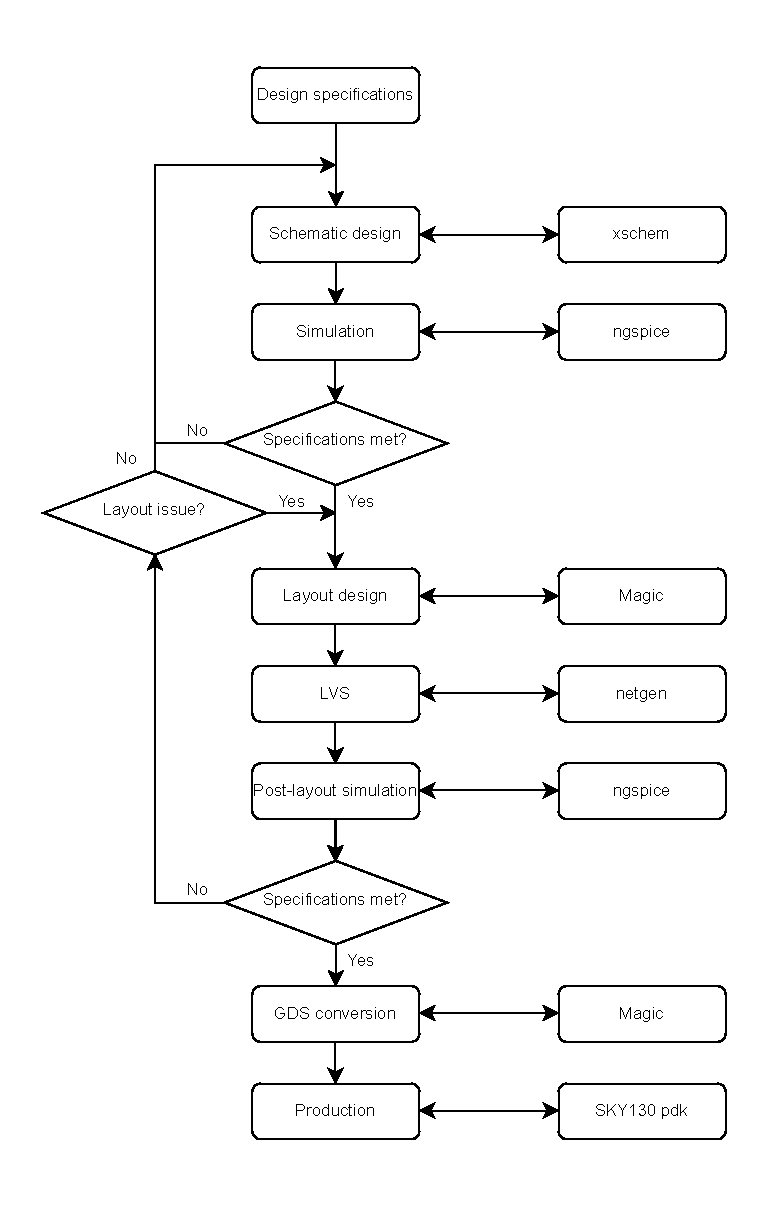
\includegraphics[width=\textwidth]{Figures/Workflow.drawio.pdf}
\caption{Analog IC Design Flow Schematic}
\label{fig:workflow_schematic}
\end{figure}


\section{Design Stages and Their Purpose}

The design stages in this workflow are as follows:

\textbf{Design Concept (Python):}
The initial stage involves formulating and modeling the idea. This stage leverages mathematical and simulation tools such as Python, along with libraries like NumPy and SciPy, to create preliminary models and validate initial concepts.

\textbf{Schematic Entry (Xschem \parencite{xschem}):}
In this stage, the design specifications are translated into a schematic diagram using tools like Xschem. Xschem simplifies the process of creating and managing schematic diagrams with its user-friendly interface.

\textbf{Simulation (ngspice) \parencite{ngspice}:}
Once the schematic is complete, the design is simulated using ngspice. This simulation tool ensures that the design operates correctly within the defined specifications, allowing for early identification and correction of any issues.

\textbf{Layout (Magic \parencite{magic}):}
The physical design stage involves drawing the geometries that will form the semiconductor device's layers. Magic is used for this purpose, providing a robust platform for creating the layout while adhering to design rules.

\textbf{Design Rule Check (DRC) (Magic):}
After the layout is complete, Magic provides an interactive DRC to validate that the layout adheres to manufacturing standards. This step is crucial for ensuring that the design can be successfully fabricated.

\textbf{Layout versus Schematic (LVS) (Netgen):}
Netgen is used to compare the LVS to ensure they match perfectly. This verification step confirms that the physical layout accurately represents the intended circuit design.

\textbf{Device and Parasitic Extraction (Magic):}
Magic also aids in the extraction of parasitic elements that occur during the layout phase. Identifying these parasitics allows for further optimization of the design, as they can impact circuit performance.

\section{Process Design Kits (PDKs)}

PDKs are vital in IC design, providing a collection of manufacturing process-specific rules, tools, and components. For this project, the SkyWater 130nm CMOS sky130 PDK \parencite{SkyWater_Technology_US_Semiconductor_Manufacturer} is utilized, offering a comprehensive suite of analog and digital design capabilities.

\section{Documentation of the Design Process in the Wiki \cite{ethz_bsse_wiki}}

Throughout this project, extensive documentation was created to aid future designers. The design process, tool presentation, installation steps, and additional resources are thoroughly detailed in the project wiki. This documentation includes:
\begin{itemize}
\item Detailed instructions on the installation and use of each tool.
\item Step-by-step guides for each stage of the design process.
\item Troubleshooting tips and best practices.
\item Links to further resources and community contributions.
\end{itemize}

For more extensive details on each tool's functions, installation, and integration with the Sky130 PDK, please refer to the wiki pages. This supplementary information provides a deeper understanding of the toolset used throughout the analog IC design process. Additionally, a small introduction to the wiki page can be found in the appendices of this report. 
%\include{Chapters/DDP}
\chapter{CMOS Inverter-Based Amplifier}
\label{chap:amplifier}

This chapter details the design, simulation, and verification of a CMOS inverter-based amplifier intended for use in a neural interface application. The amplifier utilizes open-source tools throughout the design workflow, adhering to the SkyWater 130nm CMOS PDK.
\\
This chapter presents only the results for the latest version of the amplifier design. Previous simulation results and designs can be found in Appendix \ref{AppendixB}.
\\
All files related to the amplifier design can be found in \textcite{miguelcorrea0107_2024}.

\section{Design Specifications}

The amplifier design targets the following specifications established for the first stage of neural interface applications. This amplifier is intended to serve as a pixel amplifier in an Active Pixel Sensor (APS) readout circuit on a microelectrode array. As the first stage, its role is to provide initial amplification of the signal directly at the pixel level. Further amplification typically occurs in subsequent stages.

\begin{itemize}
\item \textbf{Power Supply Voltage:} 0.5V to 1.5V (Flexibility for various neural recording setups)
\item \textbf{Input-Referred Noise:} Around 3 µV between 300 Hz to 10 kHz (Minimizes noise contribution to the neural signal)
\item \textbf{Gain:} Around 20 dB (Amplifies weak neural signals)
\item \textbf{Frequency Response:} Bandpass with flat gain between 10 Hz to 5 kHz (Focuses on the relevant frequency range of neural activity)
\item \textbf{Power Consumption:} Less than 10 µW (Low power consumption for extended device operation)
\item \textbf{Device Size:} Minimized for efficient chip area utilization
\end{itemize}

\section{Design Choices}
The final design of the amplifier is based on several strategic choices to optimize performance and minimize the footprint. 
Transistor fingering was employed to optimize the layout size, ensuring efficient use of the available area. 
Active resistors were chosen for their ability to provide high gain and low noise while maintaining a small footprint. 
Additionally, transistor-based capacitors were utilized to further reduce the overall footprint of the design. 
These design choices collectively contribute to achieving the desired specifications for the neural interface application.

\section{Schematic Design}
The amplifier design leverages a inverter architecture inspired by the work presented in \textcite{Yuan_Hierlemann_Frey_2021}.
Employing Xschem and the SkyWater 130nm PDK libraries, the schematic diagram and symbol for the circuit were created. 
Figure \ref{fig:schematic_v4} shows the schematic diagram of the amplifier design.

\begin{figure}[ht!]
\centering
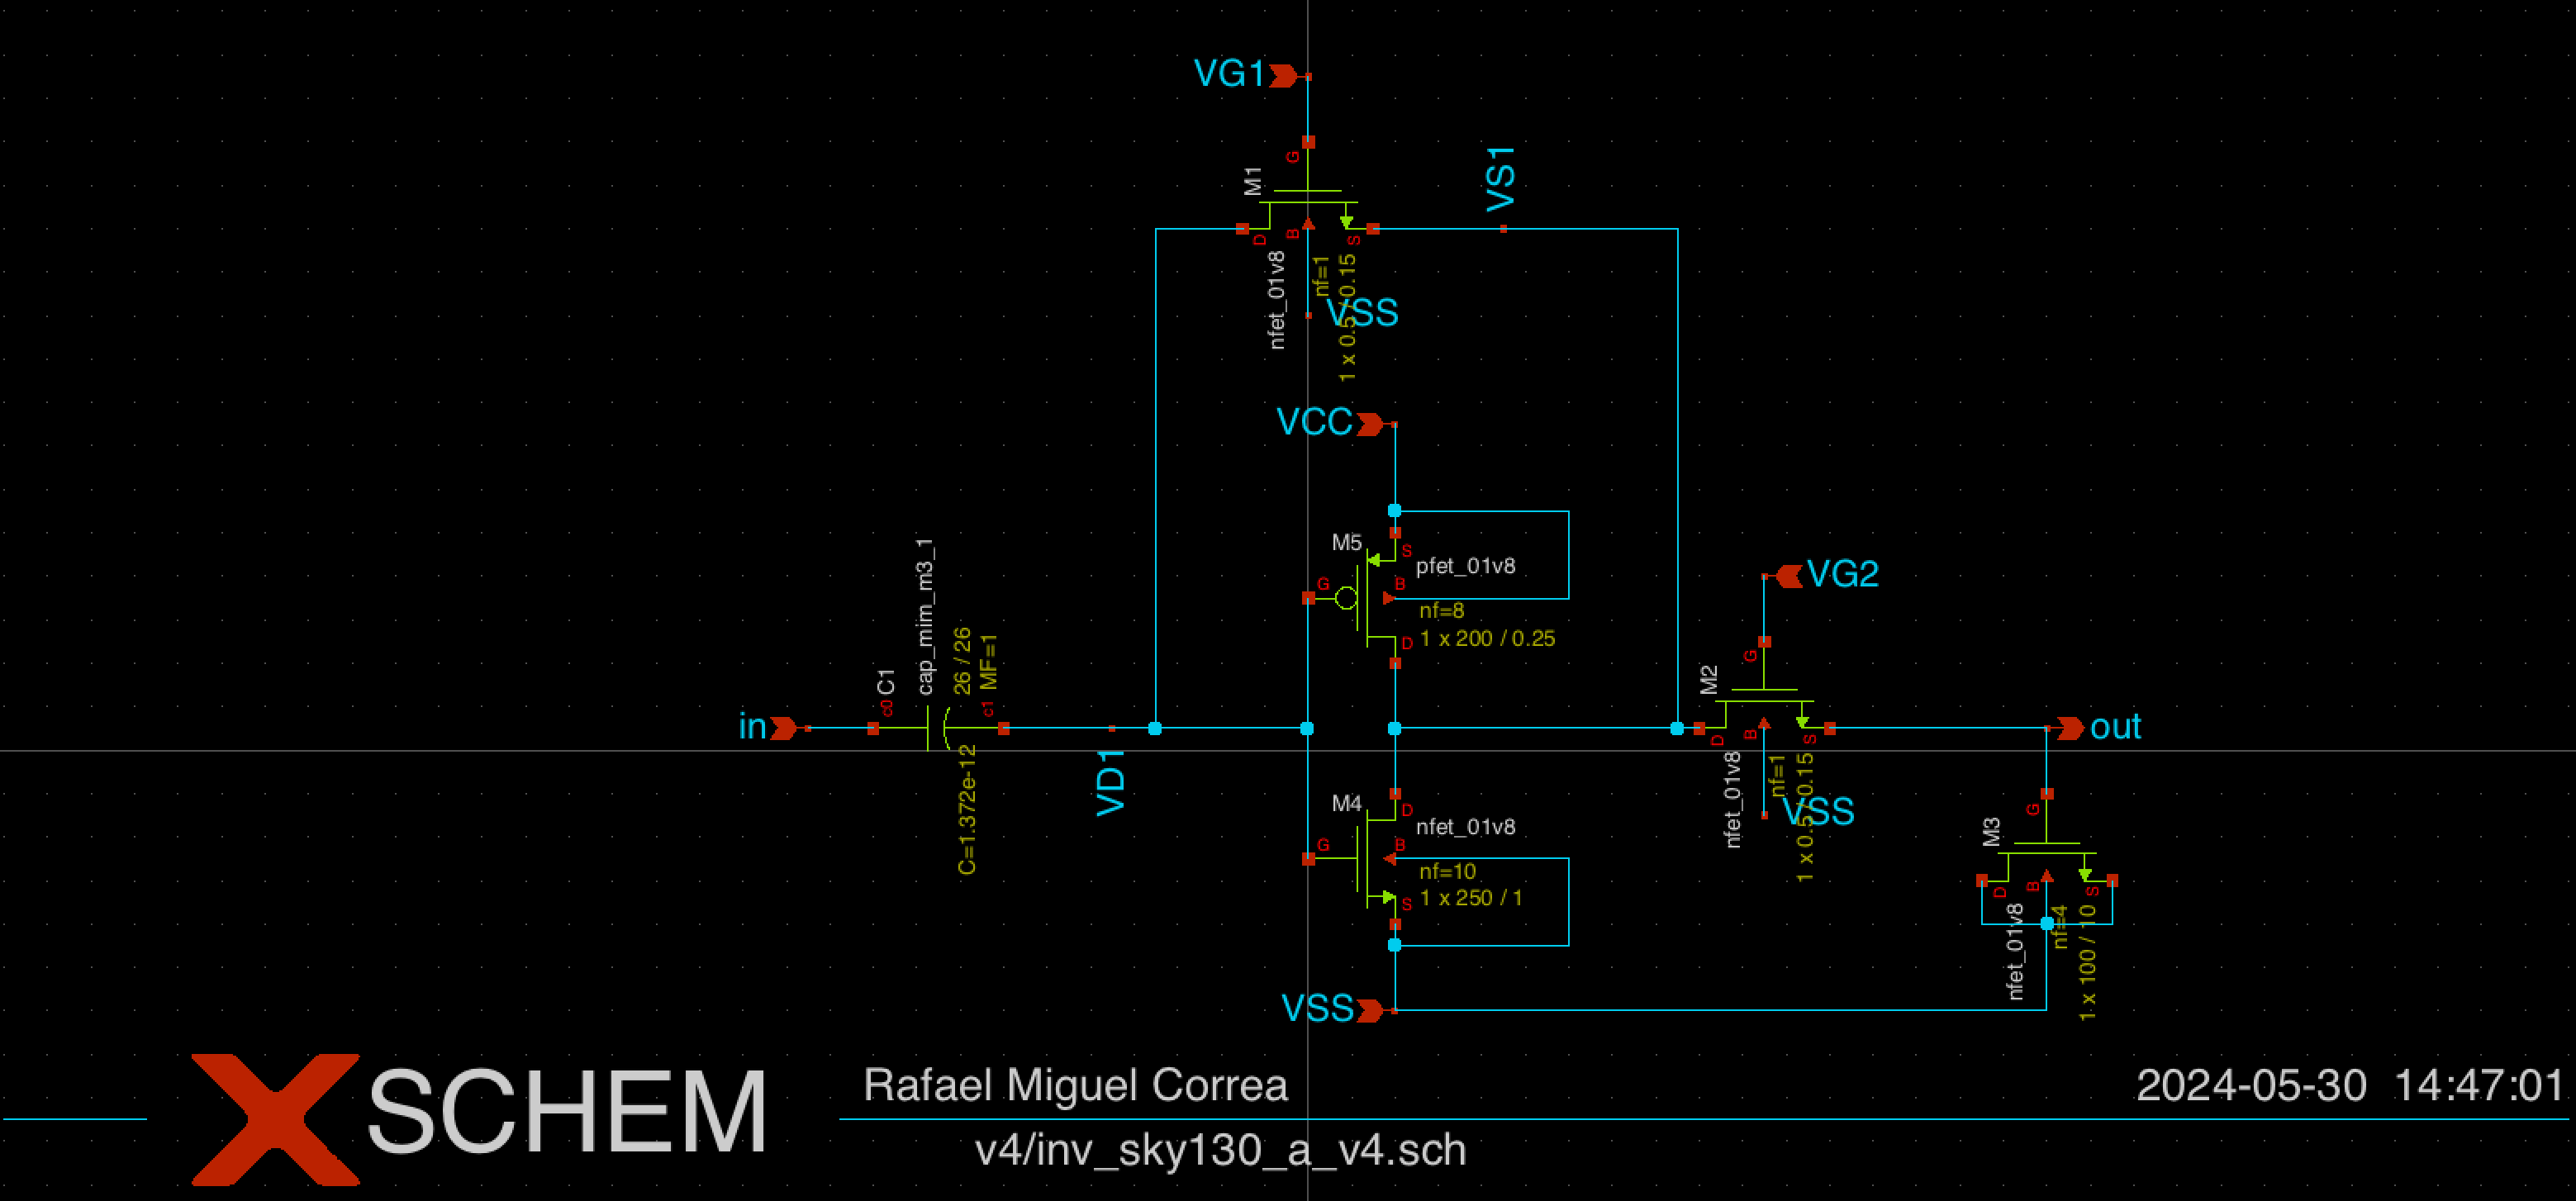
\includegraphics[width=\textwidth]{Figures/v4_schematic.png}
\caption{CMOS inverter-based amplifier schematic design.}
\label{fig:schematic_v4}
\end{figure}

\section{Simulation Results}

SPICE simulations were conducted using ngspice on a testbench (see Figure \ref{fig:testbench_v4}) to assess the amplifier's performance under various conditions. 
A test bench was designed in Xschem to automate a series of simulations, including:

\begin{itemize}
\item \textbf{Operating Point Analysis:} Determines the stable biasing condition for the transistors.
\item \textbf{AC Response:} Evaluates the amplifier's gain and frequency response (see Figure \ref{fig:frequency_response_v4}).
\item \textbf{Noise Analysis:} Estimates the input-referred noise of the amplifier (see Figure \ref{fig:noise_v4}).
\item \textbf{Transient Simulation:} Calculates the average power consumption of the amplifier during operation.
\item \textbf{DC Characteristic:} Sweeps the input voltage and measures the output voltage to determine the transfer function.
\item \textbf{Corner Simulation:} Simulates the amplifier under process, voltage, and temperature variations.
\end{itemize}

Unfortunately, Monte Carlo simulations were not performed due to time constraints and because the PDK did not provide the necessary information for the simulations.

Corner simulations showed changes in the frequency response and noise values. To address this issue, post-fabrication tuning of the amplifier will be necessary. 
Specifically, adjusting the values of $V_{g1}$ and $V_{g2}$ will ensure the amplifier meets the desired specifications.

The simulation results are as follows:

\begin{itemize}
\item \textbf{Gain:} 20.9 dB
\item \textbf{Bandwidth:} 8.9 Hz to 4.4 kHz
\item \textbf{Noise:} 5.8 µV between 300 Hz to 10 kHz
\item \textbf{Power Consumption:} 3.1 µW
\end{itemize}

\begin{figure}[ht!]
\centering
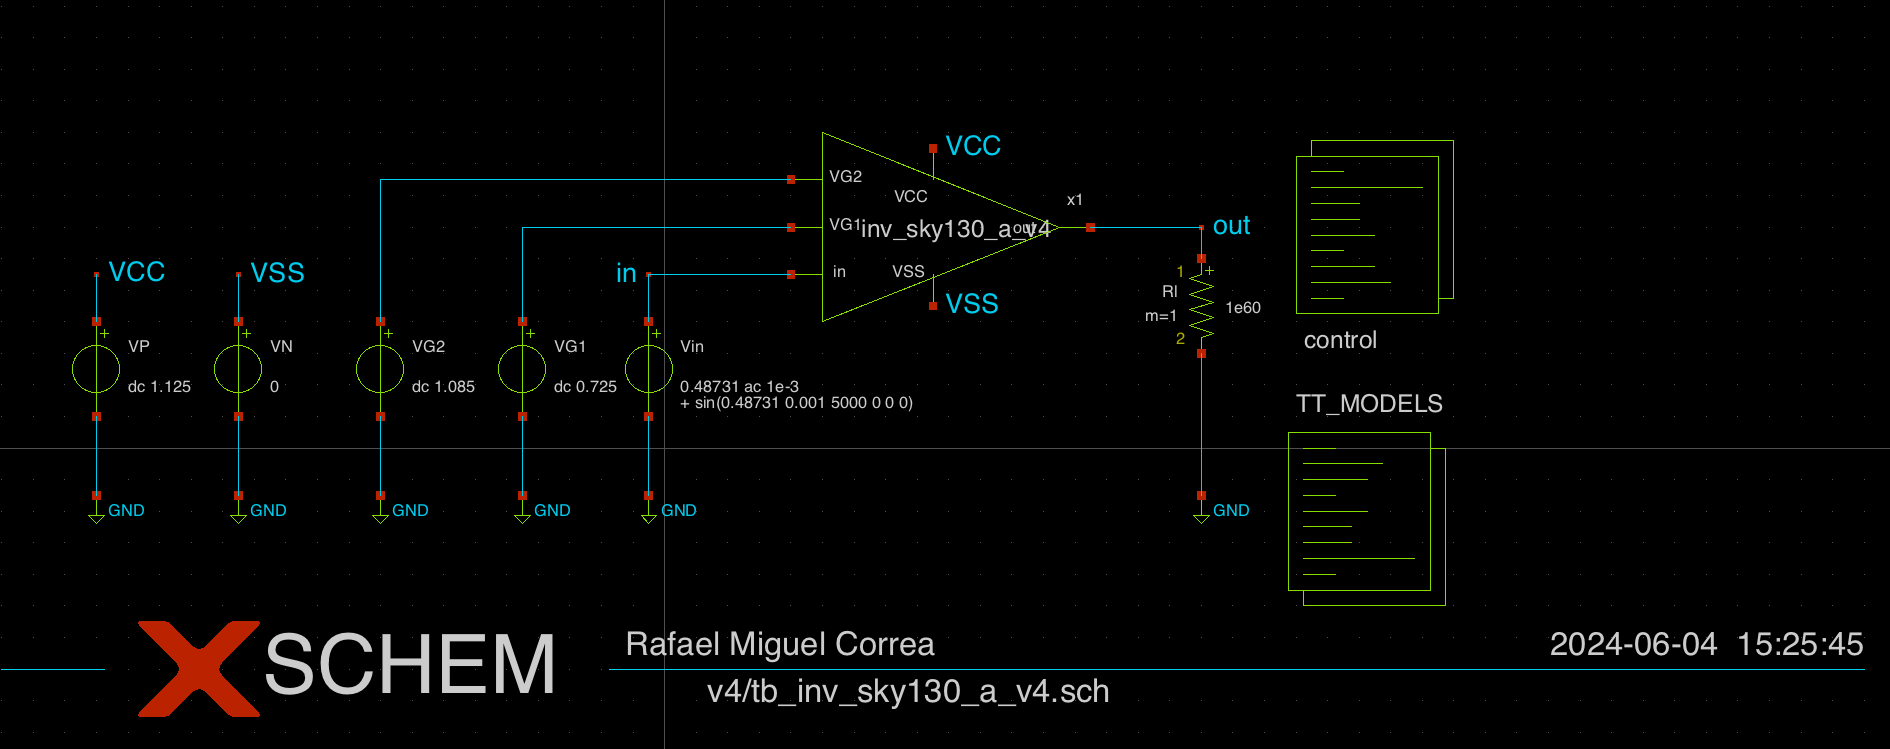
\includegraphics[width=\textwidth]{Figures/testbench.png}
\caption{CMOS inverter-based amplifier testbench.}
\label{fig:testbench_v4}
\end{figure}

\begin{figure}[ht!]
\centering
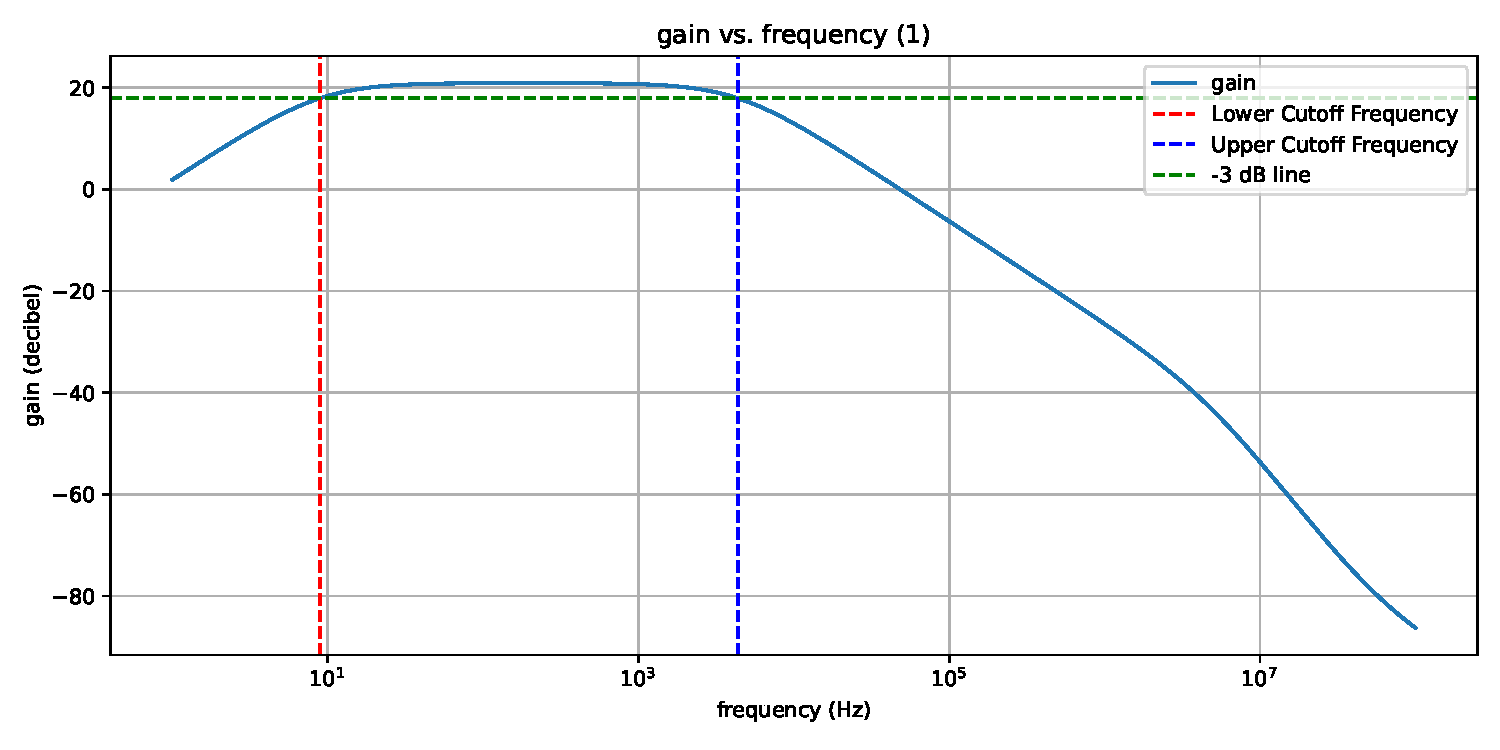
\includegraphics[width=\textwidth]{Figures/test.pdf}
\caption{CMOS inverter-based amplifier frequency response.}
\label{fig:frequency_response_v4}
\end{figure}

\begin{figure}[ht!]
\centering
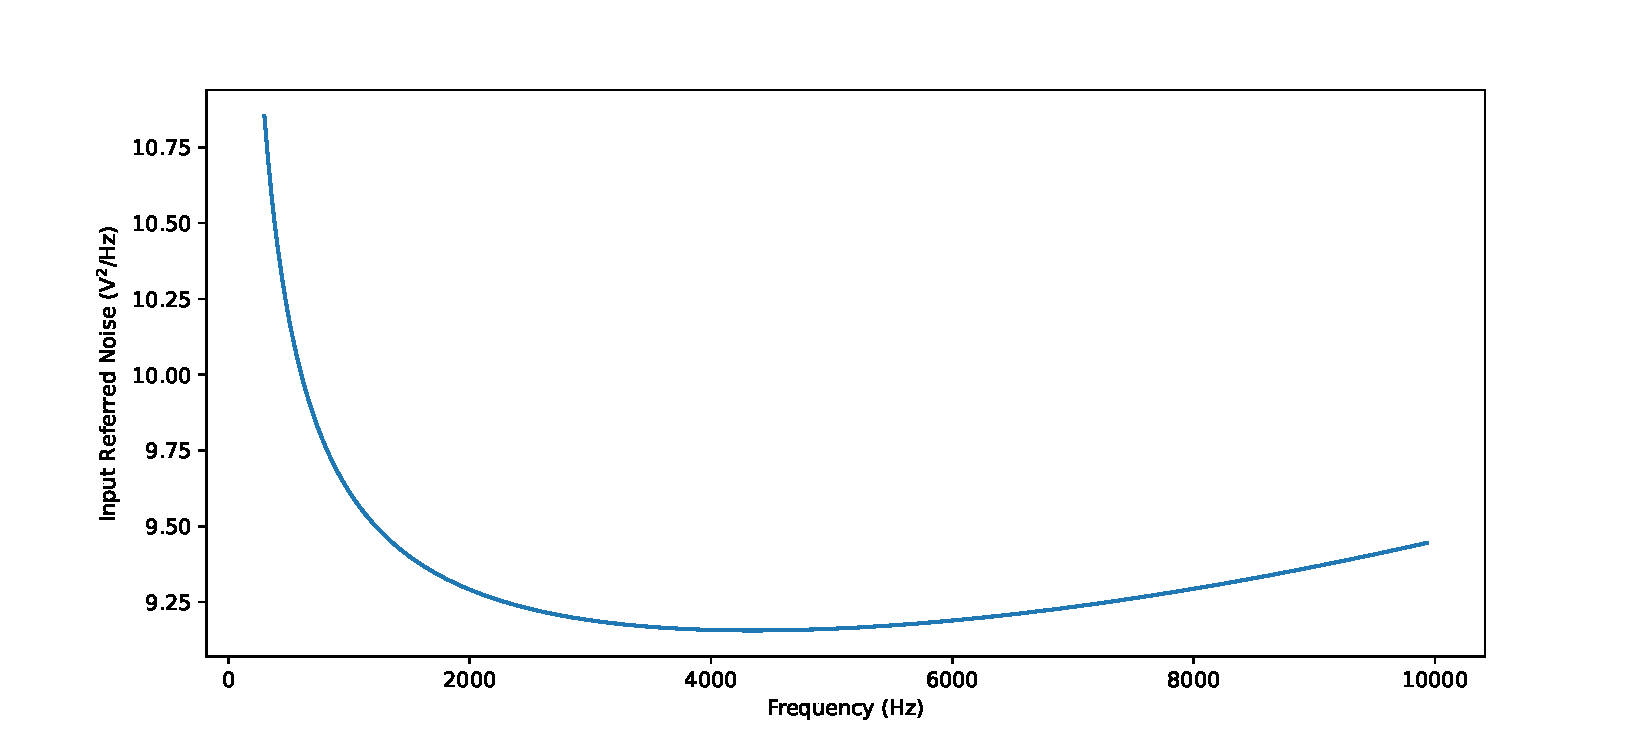
\includegraphics[width=\textwidth]{Figures/inoise_v4.pdf}
\caption{CMOS inverter-based amplifier input referred noise spectrum.}
\label{fig:noise_v4}
\end{figure}

\section{Layout Design}

Magic was used to translate the schematic design into a manufacturable layout. 
Figure \ref{fig:layout_v4} shows the layout design of the CMOS inverter-based amplifier. This layout results in:

\begin{itemize}
\item \textbf{Width:} 27.4 µm
\item \textbf{Height:} 67.95 µm
\item \textbf{Total Area:} 1861.83 µm$^2$
\end{itemize}

The layout is designed to minimize unused space and ensure efficient use of the available area.

\begin{figure}[ht!]
\centering
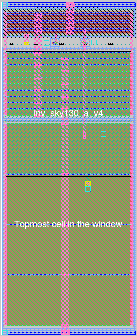
\includegraphics[width=0.6\textwidth]{Figures/final_layout.png}
\caption{CMOS inverter-based amplifier layout.}
\label{fig:layout_v4}
\end{figure}

The layout design was subjected to a rigorous DRC using Magic to ensure adherence to the SkyWater 130nm CMOS PDK foundry rules. 
This step guarantees the manufacturability of the designed layout.

Following a successful DRC check, a LVS verification was performed using Netgen. 
This process confirms that the physical layout accurately reflects the intended electrical connectivity of the schematic.

\section{Post-Layout Simulation}
Post-layout simulations were conducted using the extracted parasitic information to obtain a more realistic prediction of the amplifier's performance after fabrication. 
Table \ref{tab:specifications_comp} summarizes the post-layout simulation specifications in comparison to the desired specifications.
\\
Additionnaly, figure \ref{fig:post_layout_frequency_response} shows the frequency response of the CMOS inverter-based amplifier design post-layout, 
and figure \ref{fig:post_layout_noise} shows the noise analysis of the CMOS inverter-based amplifier design after post-layout.

\begin{table}[ht!]
    \centering
    \resizebox{\textwidth}{!}{
    \begin{tabular}{|l|c|c|}
    \hline
    \textbf{Specification} & \textbf{Desired Value} & \textbf{Final Value} \\ \hline
    Power Supply Voltage & 0.5V to 1.5V & 1.125V \\ \hline
    Input-Referred Noise & Around 3 µV between 300 Hz to 10 kHz & 6 µV between 300 Hz to 10 kHz \\ \hline
    Gain & Around 20 dB & 19.1 dB \\hline
    Frequency Response & Bandpass, 10 Hz to 5 kHz & Bandpass, 6.9 Hz to 4.7 kHz \\ \hline
    Power Consumption & Less than 10 µW & 3.2 µW \\ \hline
    Device Size & - & 1861.83 µm$^2$ \\ \hline
    \end{tabular}
    }
    \caption{Specification Comparison}
    \label{tab:specifications_comp}
\end{table}

\begin{figure}[ht!]
    \centering
    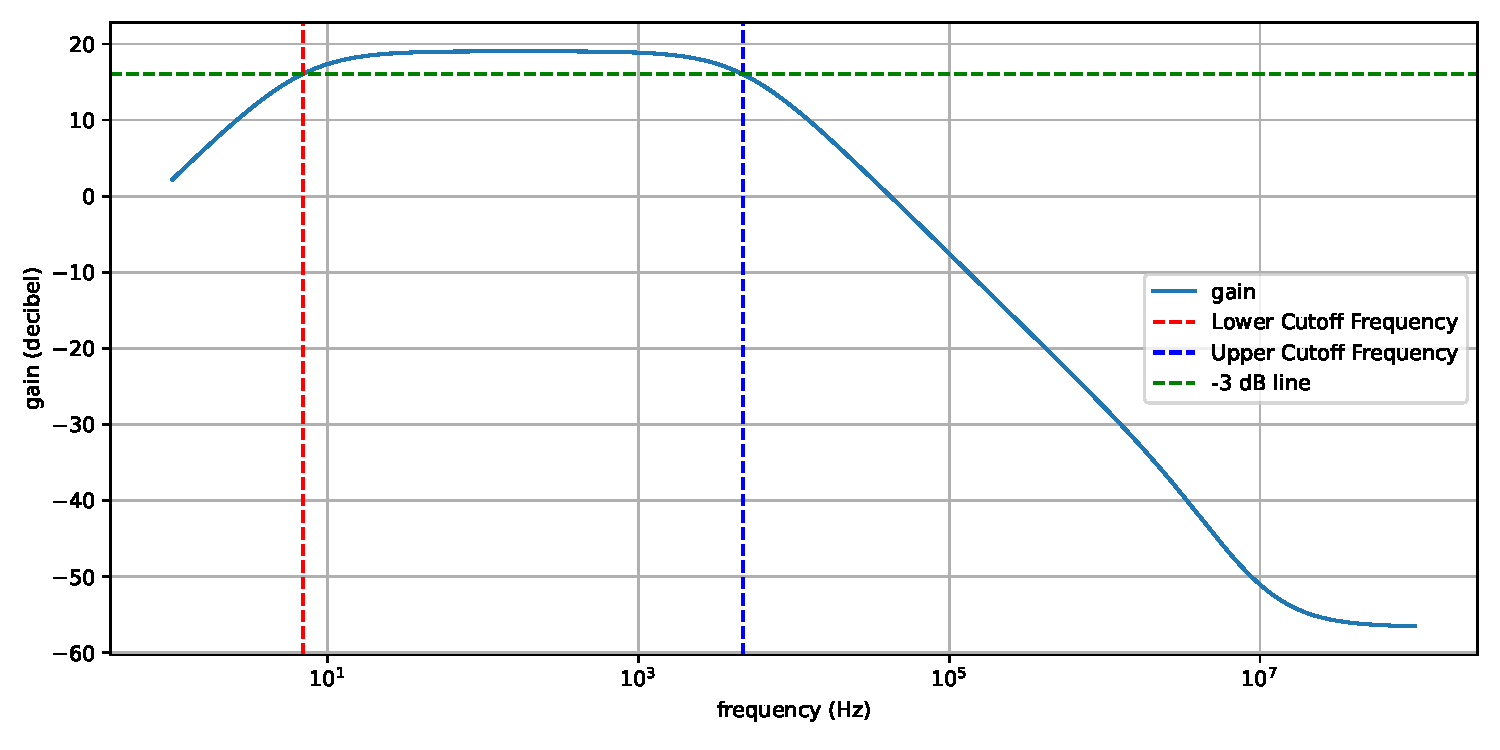
\includegraphics[width=\textwidth]{Figures/post_layout_frequency_response.pdf}
    \caption{CMOS inverter-based amplifier post-layout frequency response.}
    \label{fig:post_layout_frequency_response}
\end{figure}

\begin{figure}[ht!]
    \centering
    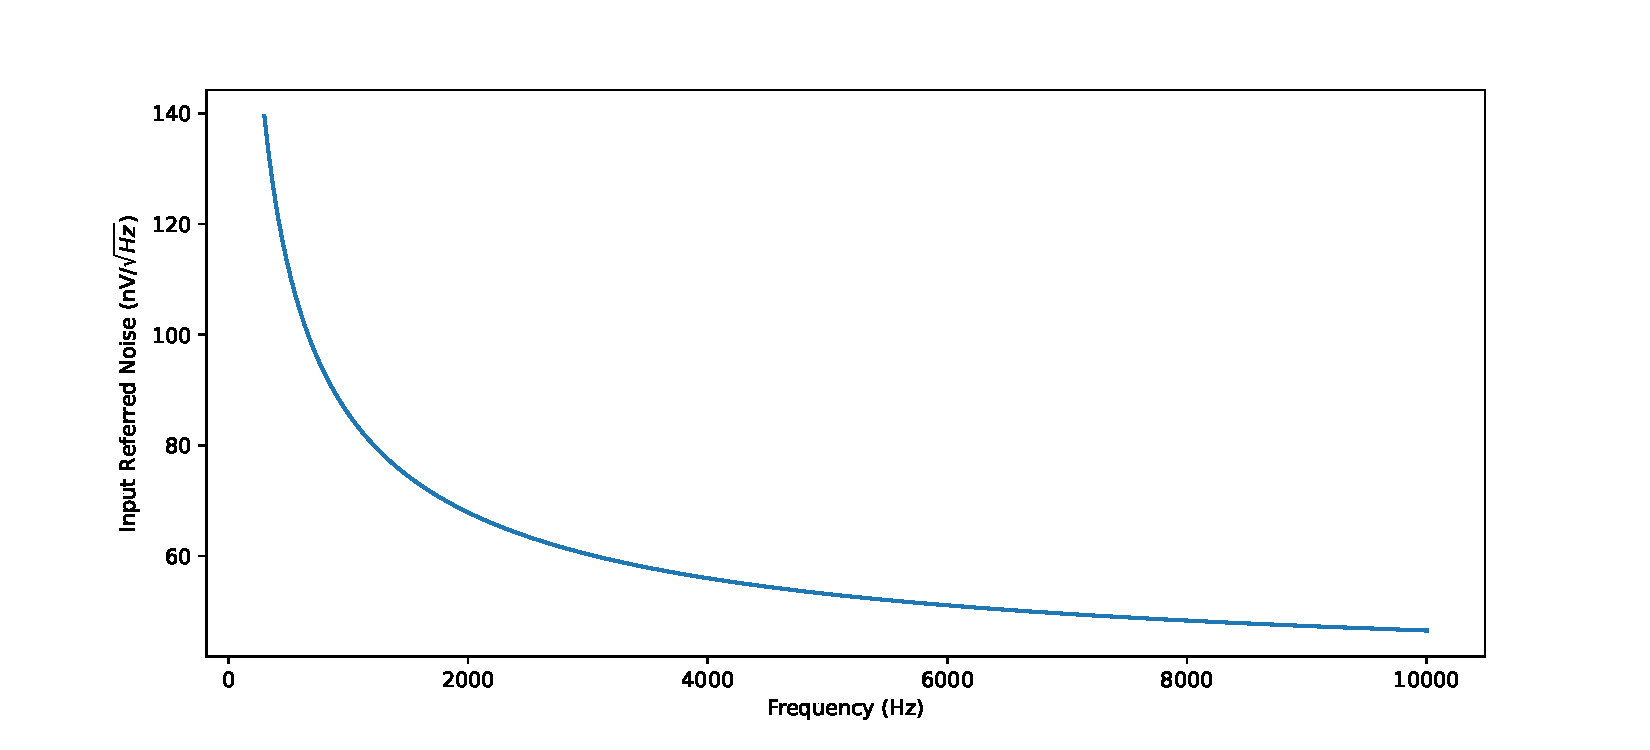
\includegraphics[width=\textwidth]{Figures/inoise_pl.pdf}
    \caption{CMOS inverter-based amplifier post-layout input referred noise spectrum.}
    \label{fig:post_layout_noise}
\end{figure}

\section{Conclusion}
The post-layout simulation results show that the amplifier meets most of the desired specifications, with slight deviations in the gain and noise levels. 
The power consumption is well within the desired range, and the frequency response, while slightly narrower, still falls within an acceptable range. 
These results indicate that the design is robust and manufacturable, with only minor adjustments needed to optimize performance further. 
The successful completion of DRC, LVS, and post-layout simulations demonstrates the readiness of the CMOS inverter-based amplifier project for fabrication, though adjustments for process variations were identified as necessary.  
\chapter{Conclusion}
\label{chap:conclusion}

This project has successfully demonstrated the feasibility and effectiveness of using open-source tools for the design of integrated circuits (ICs), specifically focusing on a CMOS inverter-based amplifier for neural interface applications. Throughout the project, we meticulously designed, simulated, and verified the amplifier, ensuring it met all specified design goals. The amplifier's design was tailored to meet stringent requirements for power supply voltage, input-referred noise, gain, frequency response, and power consumption.

A significant achievement of this project was the effective integration of several open-source tools, including Xschem, Ngspice, Magic, and Netgen, alongside the SkyWater SKY130 PDK. Extensive simulations and verifications were conducted, such as AC response, noise analysis, transient simulation, and DC characteristics, to confirm the design's reliability and performance. Additionally, the entire design process was thoroughly documented, with all project files made publicly available in a GitHub repository \cite{miguelcorrea0107_2024}, contributing to the broader open-source community.

Throughout this endeavor, we learned several important lessons. Open-source tools have reached a level of maturity that allows them to handle complex IC design tasks, albeit with a need for more setup and troubleshooting compared to proprietary tools. Leveraging the support and resources of the open-source community proved invaluable, and active participation in forums and collaboration with other designers significantly enhanced the design process. Furthermore, the iterative nature of IC design was reinforced, highlighting the importance of frequent simulations and checks, such as DRC and LVS verifications, to catch and correct errors early. Finally, the critical role of thorough documentation was underscored, not only for personal reference but also for knowledge sharing. Detailed records of each design step and decision facilitate future projects and contribute to the collective knowledge base.

Despite the project's successes, several challenges were encountered and overcome. Ensuring compatibility between different tools required meticulous attention, particularly when integrating outputs and inputs across various software. Additionally, while open-source tools are powerful, they sometimes lack the advanced functionalities found in proprietary tools, such as sophisticated simulation models and advanced layout automation. This limitation necessitated creative problem-solving and workarounds to achieve the desired design goals.

This project paves the way for several future endeavors and improvements. Incorporating more advanced design features and exploring other types of amplifiers or ICs can expand the scope and utility of open-source IC design. Moving from design and simulation to the actual fabrication and testing of the amplifier would be a logical next step, providing real-world validation of the design.

In conclusion, this project underscores the potential of open-source tools in the field of IC design, particularly for the BEL group. By achieving our design goals and documenting the process comprehensively, we aim to contribute valuable knowledge and resources to the field. Open-source design not only democratizes access to advanced technology but also fosters innovation through collaboration and shared learning. The successful outcomes of this project lay a solid foundation for future explorations and advancements in open-source IC design. 

%----------------------------------------------------------------------------------------
%	THESIS CONTENT - sNDICES
%----------------------------------------------------------------------------------------

\appendix % Cue to tell LaTeX that the following "chapters" are Appendices

% Include the appendices of the thesis as separate files from the Appendices folder
% Uncomment the lines as you write the Appendices

\chapter{Simulation Results}
\label{AppendixA}

This appendix documents the evolution of the CMOS inverter-based amplifier design through multiple versions. Each version addresses specific design challenges and improvements, validated through extensive simulations. Detailed results and schematics for each version are provided to illustrate the design iterations and their impact on performance.

\section{Version 1}

The first version of the design was based on the calculation of the transfer function using the DPSFG (Driving Point Signal Flow Graph) technique (see \textcite{Schmid_Huber_2018}). 
More details about this calculation can be found in the inv$\_$parameters.ipynb file on the GitHub repository \cite{miguelcorrea0107_2024}. 
This version had to be revised to incorporate active resistors due to size constraints.
\\
Figure \ref{fig:v1_schematic} shows the schematic of Version 1. 
The simulation results for this version are summarized in Table \ref{tab:v1_sim_results}.
\begin{figure}[ht!]
    \centering
    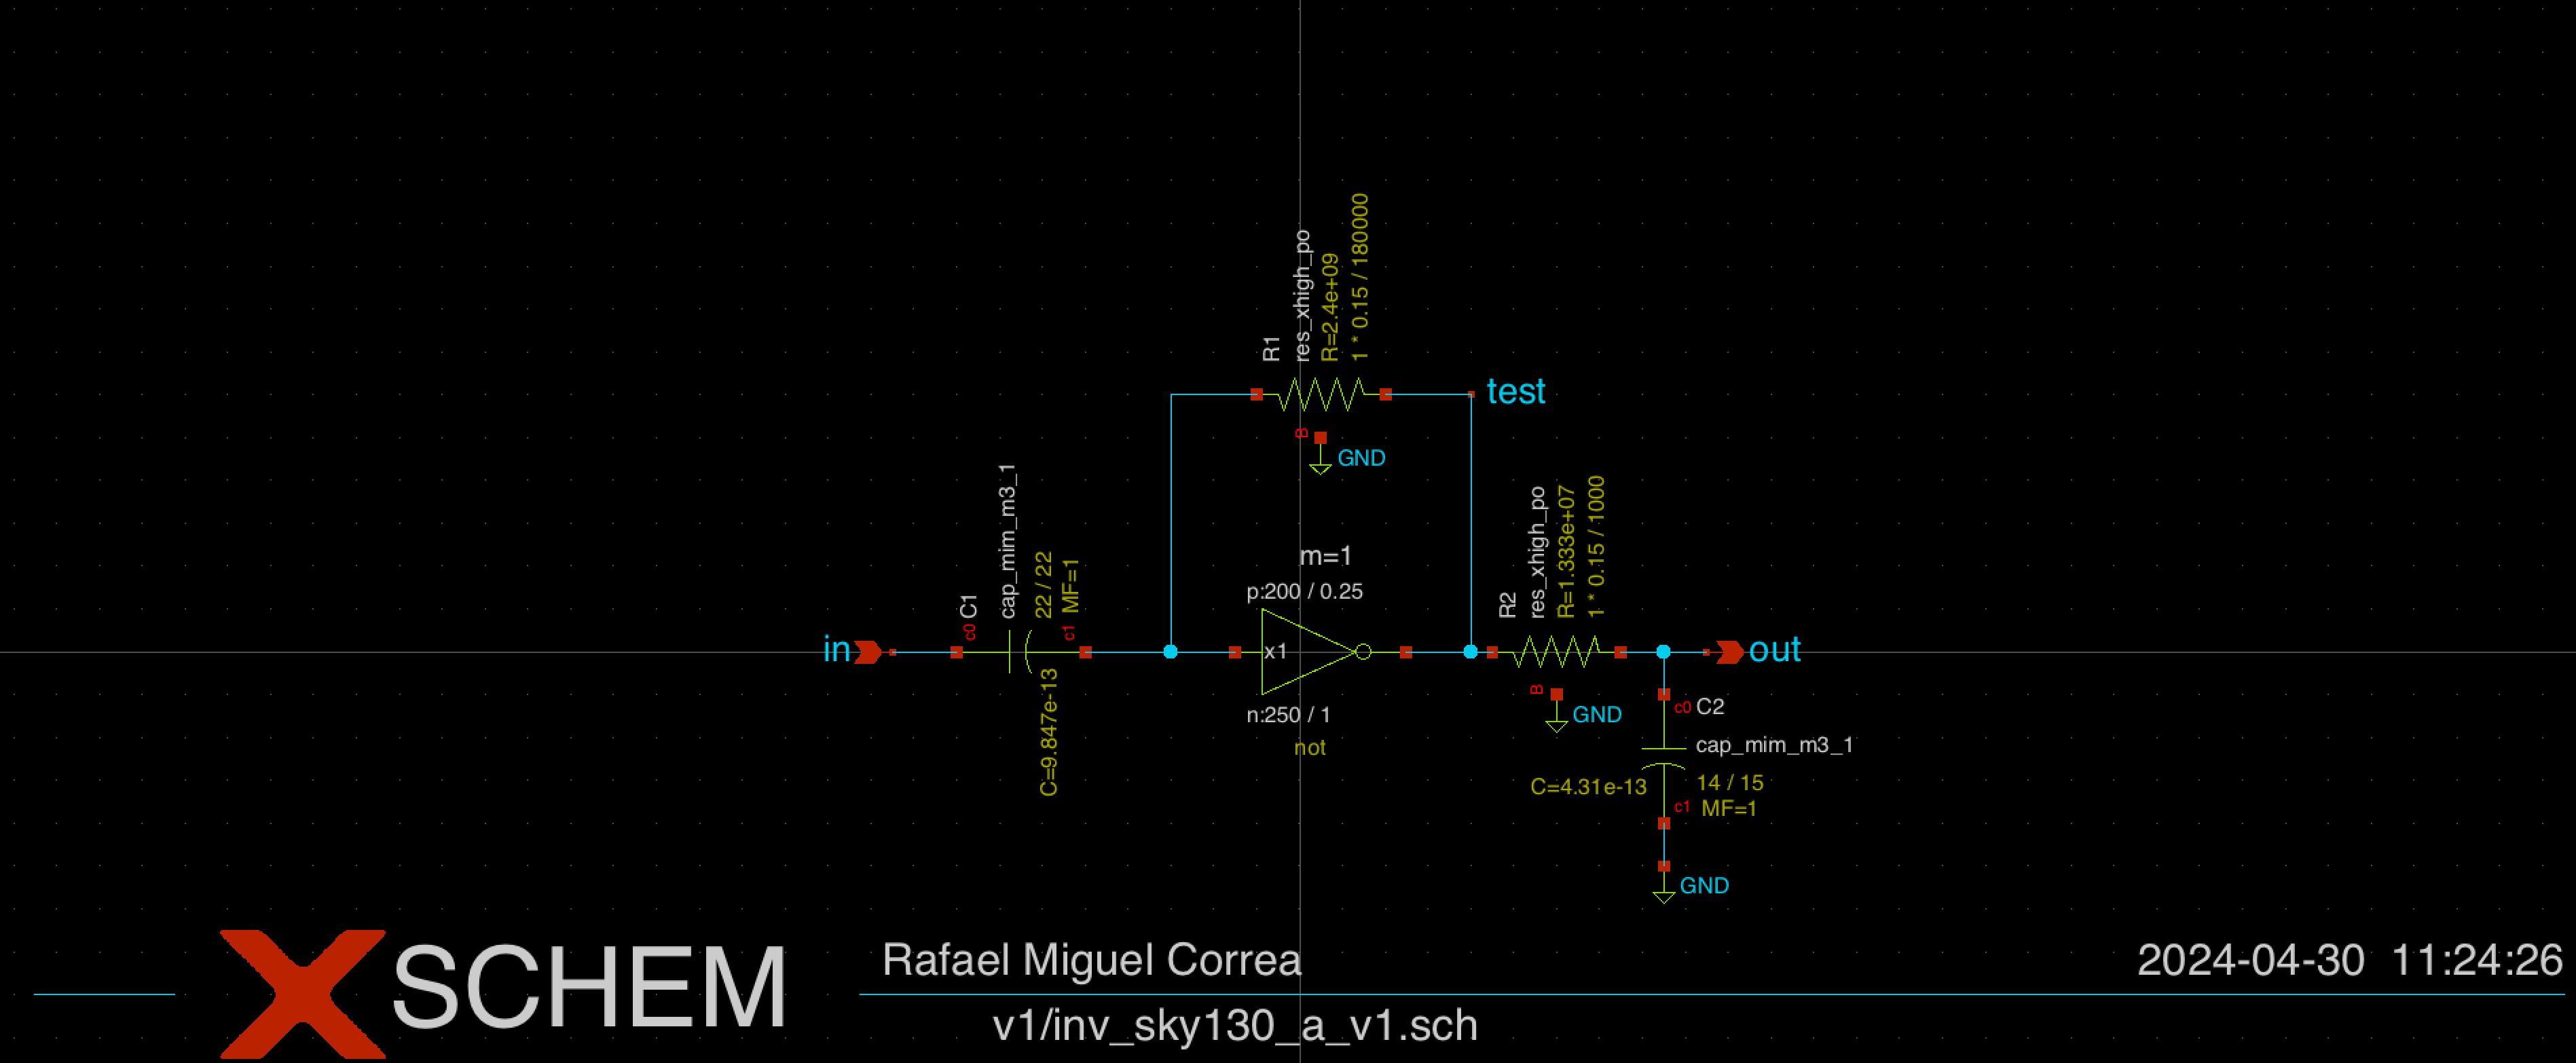
\includegraphics[width=\textwidth]{Figures/v1_schematic.png}
    \caption{Schematic of Version 1 of the CMOS inverter-based amplifier design.}
    \label{fig:v1_schematic}
\end{figure}

\begin{landscape}
\begin{table}[!ht]
    \centering
    \begin{adjustbox}{max width=\linewidth}
    \begin{tabular}{|c|c|c|c|c|c|c|c|c|c|c|c|c|c|c|}
        \hline
        \textbf{Vdd} & 1.5 & 1.25 & 1.125 & 1.125 & 1.125 & 1.125 & 1.125 & 1.125 & 1.125 & 1.125 & 1.125 & 1.125 & 1.125 & 1.125 \\ \hline
         \textbf{Wn} & 20.0 & 40.0 & 50.0 & 50.0 & 250.0 & 250.0 & 250.0 & 250.0 & 250.0 & 250.0 & 250.0 & 250.0 & 250.0 & 250.0 \\ \hline
            \textbf{Ln} & 0.15 & 0.15 & 0.15 & 0.15 & 1.0 & 1.0 & 1.0 & 1.0 & 1.0 & 1.0 & 1.0 & 1.0 & 1.0 & 1.0 \\ \hline
            \textbf{Wp} & 40.0 & 80.0 & 100.0 & 100.0 & 200.0 & 200.0 & 200.0 & 200.0 & 200.0 & 200.0 & 200.0 & 200.0 & 200.0 & 200.0 \\ \hline
            \textbf{Lp} & 0.15 & 0.15 & 0.15 & 0.15 & 0.25 & 0.25 & 0.25 & 0.25 & 0.25 & 0.25 & 0.25 & 0.25 & 0.25 & 0.25 \\ \hline
            \textbf{Wr1} & 1.0 & 1.0 & 1.0 & 1.0 & 1.0 & 1.0 & 0.15 & 0.15 & 0.15 & 0.15 & 0.15 & 0.15 & 0.15 & 0.15 \\ \hline
            \textbf{Lr1} & 30.0 & 50.0 & 90.0 & 90.0 & 90.0 & 90.0 & 100.0 & 100.0 & 250.0 & 300.0 & 300.0 & 25000.0 & 200000.0 & 200000.0 \\ \hline
            \textbf{R1 (in KOhms)} & 60.0 & 100.0 & 180.0 & 180.0 & 180.0 & 180.0 & 1333.333 & 1333.333 & 3333.333 & 4000.0 & 4000.0 & 333333.3 & 2666667.0 & 2666667.0 \\ \hline
            \textbf{Wr2} & 1.0 & 1.0 & 1.0 & 1.0 & 1.0 & 1.0 & 0.15 & 0.15 & 0.3 & 0.4 & 0.15 & 0.15 & 0.15 & 0.15 \\ \hline
            \textbf{Lr2} & 50.0 & 50.0 & 50.0 & 50.0 & 50.0 & 50.0 & 1.0 & 10.0 & 1.0 & 20.0 & 10.0 & 500.0 & 1000.0 & 1000.0 \\ \hline
            \textbf{R2 (in KOhms)} & 100.0 & 100.0 & 100.0 & 100.0 & 100.0 & 100.0 & 13.33333 & 133.33329999999998 & 6.666667 & 100.0 & 133.33329999999998 & 6666.667 & 13333.33 & 13333.33 \\ \hline
            \textbf{Wc1} & 0.0 & 0.0 & 0.0 & 0.0 & 0.0 & 0.0 & 22.0 & 22.0 & 100.0 & 100.0 & 170.0 & 42.0 & 13.0 & 22.0 \\ \hline
            \textbf{Lc1} & 0.0 & 0.0 & 0.0 & 0.0 & 0.0 & 0.0 & 22.0 & 22.0 & 100.0 & 100.0 & 170.0 & 42.0 & 13.0 & 22.0 \\ \hline
            \textbf{MFc1} & 0.0 & 0.0 & 0.0 & 0.0 & 0.0 & 0.0 & 1.0 & 1.0 & 1.0 & 1.0 & 1.0 & 1.0 & 1.0 & 1.0 \\ \hline
            \textbf{C1 (in PF)} & 0.0 & 0.0 & 0.0 & 0.0 & 0.0 & 0.0 & 0.98472 & 0.98472 & 20.076 & 20.076 & 57.929199999999994 & 3.55992 & 0.34787999999999997 & 0.98472 \\ \hline
            \textbf{Wc2} & 15.0 & 15.0 & 14.0 & 70.0 & 70.0 & 55.0 & 50.0 & 50.0 & 100.0 & 170.0 & 250.0 & 47.0 & 14.0 & 14.0 \\ \hline
            \textbf{Lc2} & 15.0 & 15.0 & 13.0 & 60.0 & 60.0 & 55.0 & 50.0 & 50.0 & 100.0 & 170.0 & 250.0 & 48.0 & 15.0 & 15.0 \\ \hline
            \textbf{MFc2} & 6.0 & 6.0 & 6.0 & 6.0 & 6.0 & 5.0 & 1.0 & 1.0 & 1.0 & 1.0 & 1.0 & 1.0 & 1.0 & 1.0 \\ \hline
            \textbf{C2 (in PF)} & 2.768 & 2.768 & 2.246 & 50.699999999999996 & 50.6964 & 30.459000000000003 & 5.038 & 5.038 & 20.076 & 57.929199999999994 & 125.19000000000001 & 4.5481 & 0.43102 & 0.43102 \\ \hline
            \textbf{Vdc (in MV)} & 705.2 & 590.0999999999999 & 538.0 & 538.0 & 448.66 & 448.66 & 448.66 & 448.66 & 448.66 & 448.66 & 448.66 & 448.66 & 448.66 & 448.66 \\ \hline
            \textbf{Gain (in DB)} & 20.51506 & 20.22268 & 20.17452 & 20.17452 & 23.82489 & 23.82489 & 14.74058 & 3.778642 & 31.82523 & 24.36886 & 20.45644 & 22.77707 & 7.736271 & 16.13267 \\ \hline
            \textbf{Lower Cut-Off Frequency (in Hz)} & 0.0 & 0.0 & 0.0 & 0.0 & 0.0 & 0.0 & 158489.3 & 62661.39 & 19364.22 & 8147.043 & 2213.095 & 606.7363 & 162.5549 & 150.6607 \\ \hline
            \textbf{Upper Cut-Off Frequency (in KHz)} & 525.0492 & 489.2721 & 519.937 & 23.02707 & 12.94196 & 21.51295 & 403645.4 & 411149.7 & 41399.97 & 22233.1 & 10000.0 & 3706.807 & 10715.19 & 10665.96 \\ \hline
            \textbf{Noise In (uV)} & 15.43656 & 9.761662 & 8.460034 & 8.460322 & 2.832653 & 2.832481 & 136.7781 & 136.7782 & 3.920957 & 3.632231 & 2.871612 & 3.833044 & 27.8819 & 11.58093 \\ \hline
            \textbf{Power (in UW)} & 161.3881 & 30.48936 & 9.831864 & 9.831872 & 2.794655 & 2.794644 & 2.794441 & 2.794441 & 2.794434 & 2.794422 & 2.794327 & 2.794165 & 2.794416 & 2.794374 \\ \hline
    \end{tabular}
    \end{adjustbox}
    \caption{Simulation results for Version 1 of the CMOS inverter-based amplifier design.}
    \label{tab:v1_sim_results}
\end{table}
\end{landscape}

\section{Version 2}
This version incorporated active resistors but encountered issues due to incorrect biasing of the resistors.
\\
Figure \ref{fig:v2_schematic} shows the schematic of Version 2. 
The simulation results for this version are summarized in Table \ref{tab:v2_sim_results}.
\begin{figure}[ht!]
    \centering
    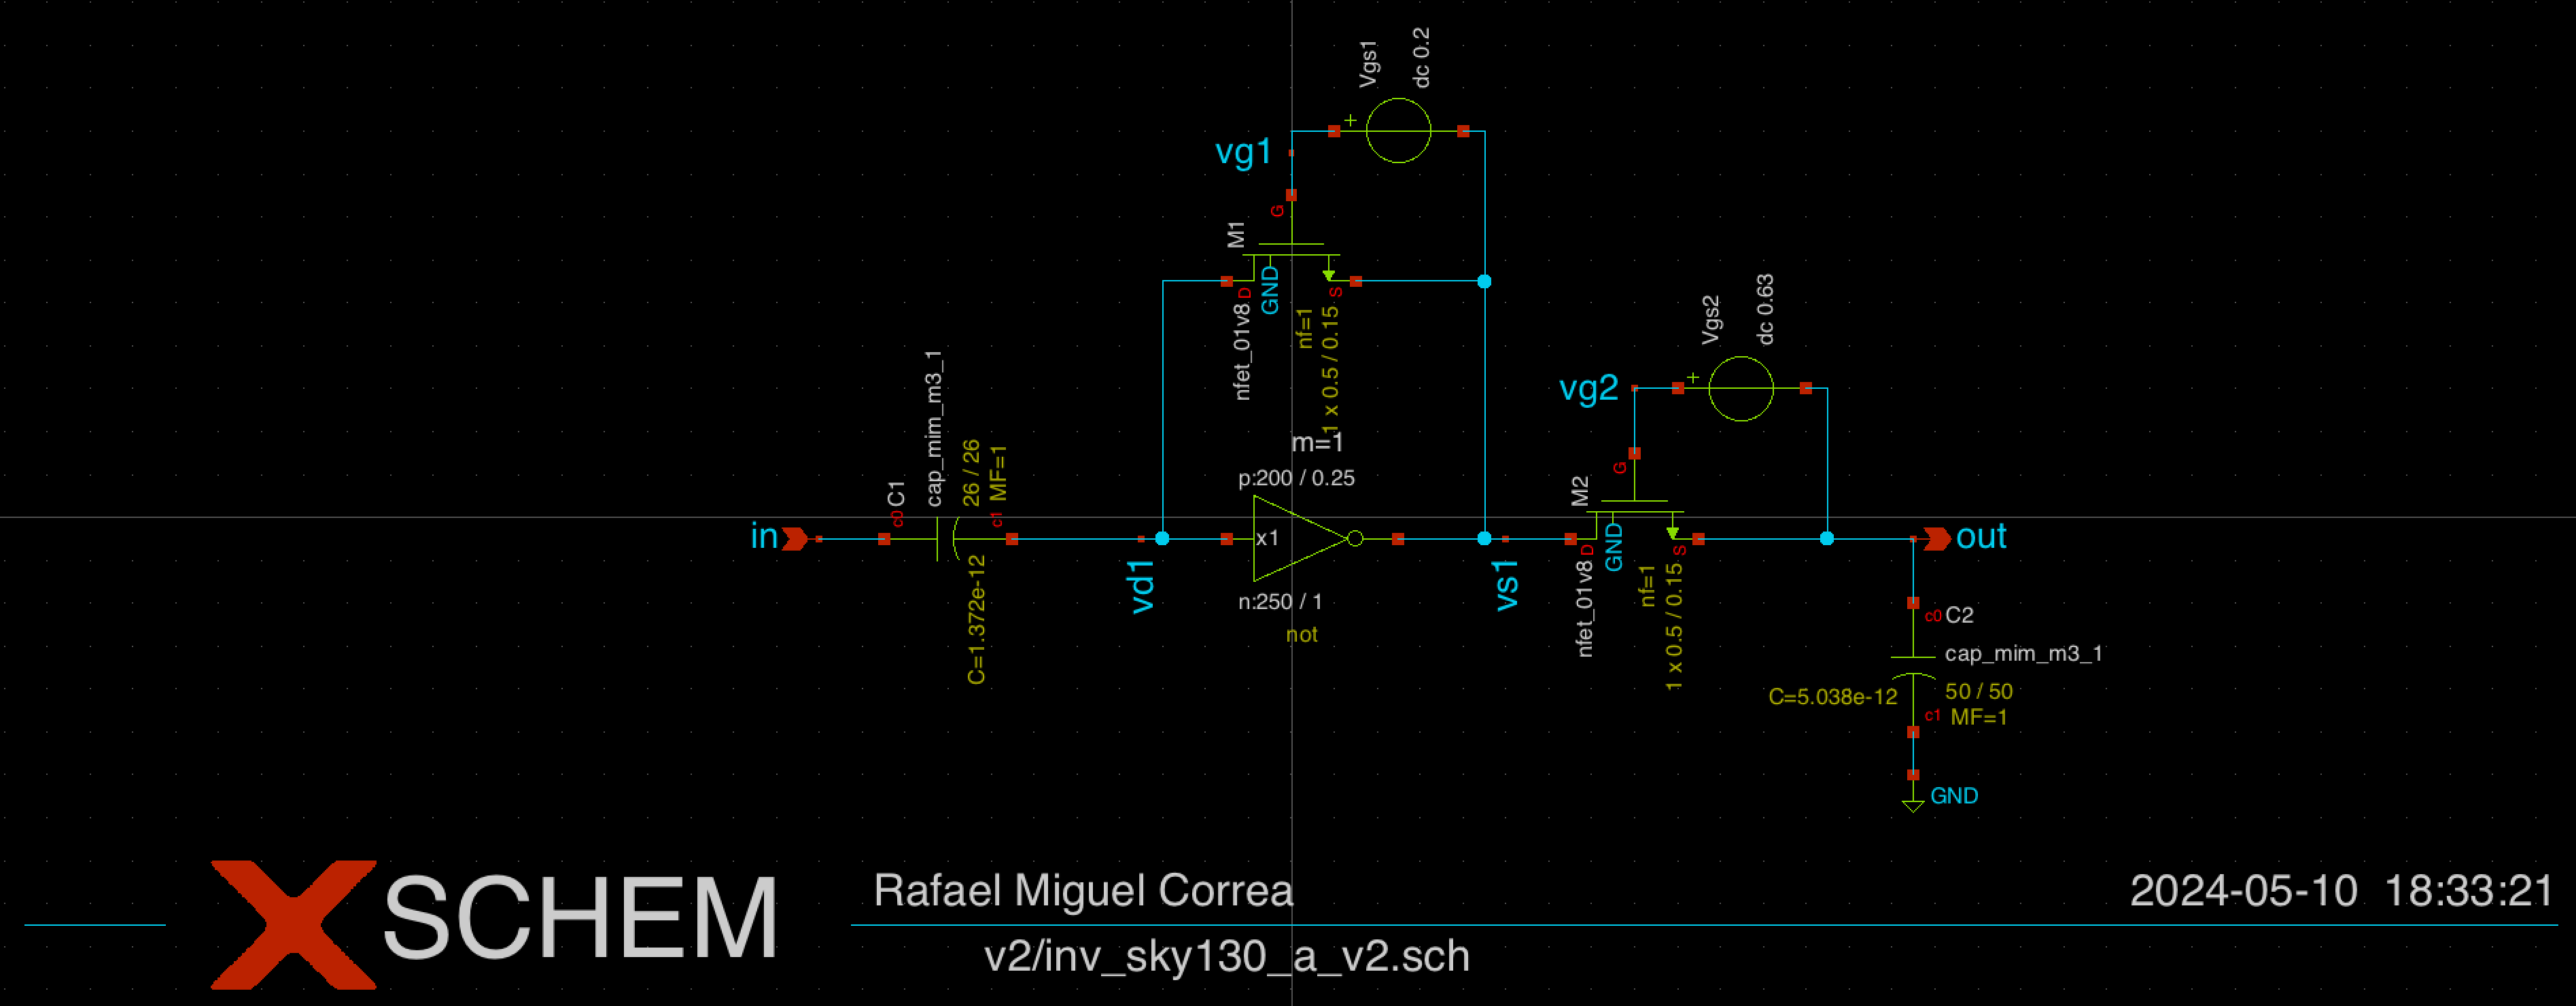
\includegraphics[width=\textwidth]{Figures/v2_schematic.png}
    \caption{Schematic of Version 2 of the CMOS inverter-based amplifier design.}
    \label{fig:v2_schematic}
\end{figure}

%\begin{landscape}
\begin{table}[!ht]
    \centering
    \begin{adjustbox}{max width=\linewidth}
    \begin{tabular}{|c|c|c|c|c|c|}
    \hline
        \textbf{Vdd} & 1.125 & 1.125 & 1.125 & 1.125 & 1.125 \\ \hline
        \textbf{Wn} & 250.0 & 250.0 & 250.0 & 250.0 & 250.0 \\ \hline
        \textbf{Ln} & 1.0 & 1.0 & 1.0 & 1.0 & 1.0 \\ \hline
        \textbf{Wp} & 200.0 & 200.0 & 200.0 & 200.0 & 200.0 \\ \hline
        \textbf{Lp} & 0.25 & 0.25 & 0.25 & 0.25 & 0.25 \\ \hline
        \textbf{R1\_Wn} & 0.5 & 0.5 & 0.5 & 0.5 & 0.5 \\ \hline
        \textbf{R1\_Ln} & 0.15 & 0.15 & 0.15 & 0.15 & 0.15 \\ \hline
        \textbf{R1\_Vgs} & 0.35 & 0.3 & 0.26 & 0.26 & 0.2 \\ \hline
        \textbf{R2\_Wn} & 0.5 & 0.5 & 0.5 & 0.5 & 0.5 \\ \hline
        \textbf{R2\_Ln} & 0.15 & 0.15 & 0.15 & 0.15 & 0.15 \\ \hline
        \textbf{R2\_Vgs} & 0.5 & 0.55 & 0.6 & 0.6 & 0.63 \\ \hline
        \textbf{Wc1} & 22.0 & 22.0 & 26.0 & 26.0 & 26.0 \\ \hline
        \textbf{Lc1} & 22.0 & 22.0 & 26.0 & 26.0 & 26.0 \\ \hline
        \textbf{MFc1} & 1.0 & 1.0 & 1.0 & 1.0 & 1.0 \\ \hline
        \textbf{C1 (in pF)} & 0.98472 & 0.98472 & 1.37176 & 1.37176 & 1.37176 \\ \hline
        \textbf{Wc2} & 14.0 & 14.0 & 30.0 & 35.0 & 50.0 \\ \hline
        \textbf{Lc2} & 15.0 & 15.0 & 30.0 & 35.0 & 50.0 \\ \hline
        \textbf{MFc2} & 1.0 & 1.0 & 1.0 & 1.0 & 1.0 \\ \hline
        \textbf{C2 (in pF)} & 0.43102 & 0.43102 & 1.8228 & 2.4766000000000004 & 5.038 \\ \hline
        \textbf{Vdc (in mV)} & 450.0 & 450.0 & 450.0 & 450.0 & 448.66 \\ \hline
        \textbf{gain (in dB)} & 18.08885 & 18.51345 & 20.90514 & 20.89836 & 20.8709 \\ \hline
        \textbf{lower cut-off frequency (in Hz)} & 220.2926 & 72.4436 & 33.72873 & 33.72873 & 20.6063 \\ \hline
        \textbf{upper cut-off frequency (in Hz)} & 4886.524 & 17701.09 & 15135.61 & 11168.63 & 10069.32 \\ \hline
        \textbf{noise in (uV)} & 14.97764 & 8.773817 & 5.699407 & 5.699722 & 5.444804 \\ \hline
        \textbf{power (in uW)} & 2.792742 & 2.787491 & 2.777074 & 2.777075 & 2.747301 \\ \hline
    \end{tabular}
    \end{adjustbox}
    \caption{Simulation results for Version 2 of the CMOS inverter-based amplifier design.}
    \label{tab:v2_sim_results}
\end{table}
%\end{landscape}

\section{Version 3}
The third version fixed the biasing of the active resistors, addressing the issues found in the previous version.
\\
Figure \ref{fig:v3_schematic} shows the schematic of Version 3. 
The simulation results for this version are summarized in Table \ref{tab:v3_sim_results}.
\begin{figure}[ht!]
    \centering
    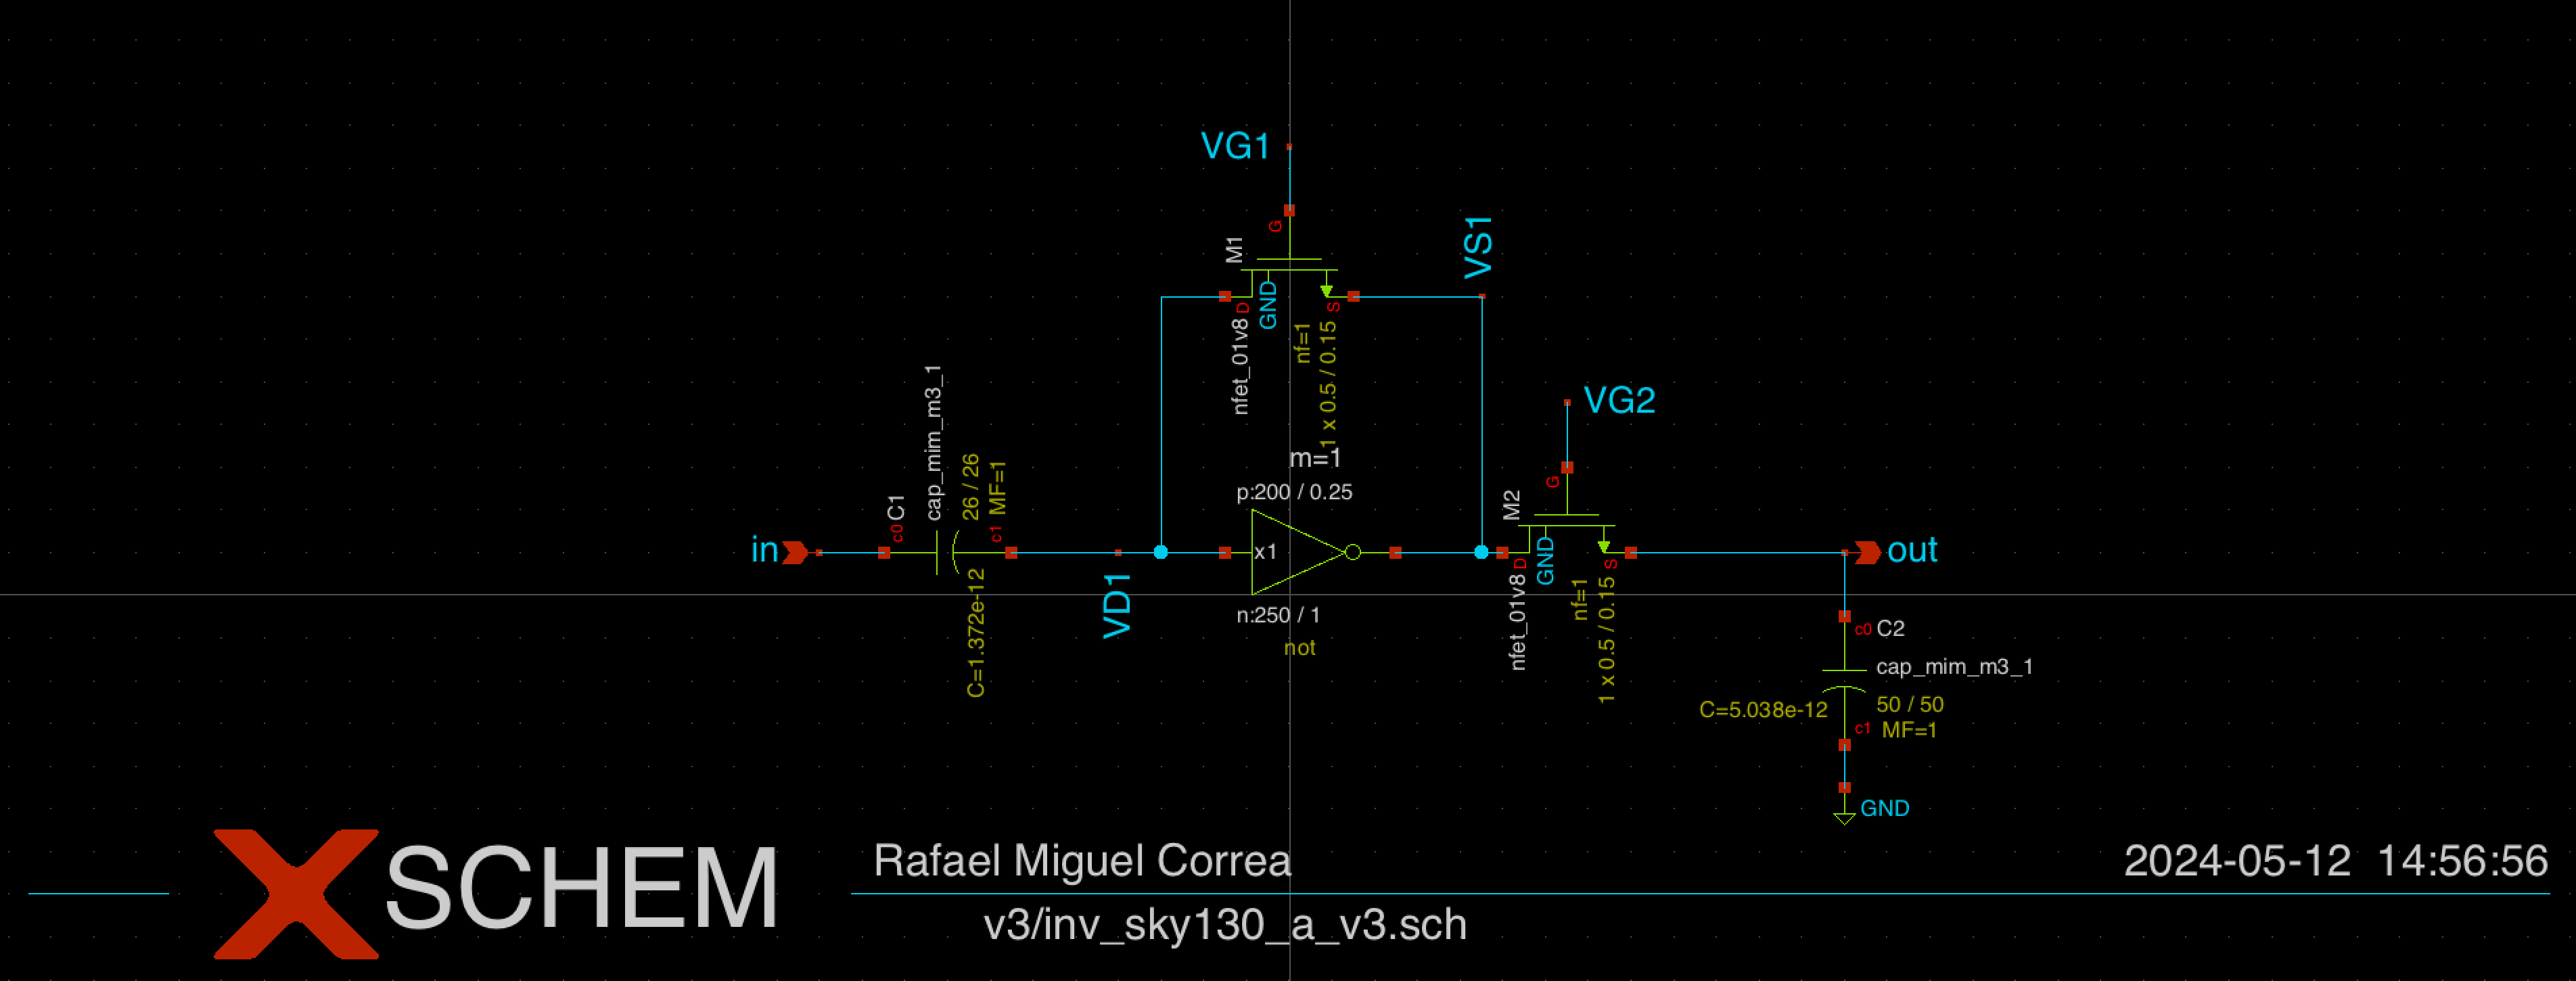
\includegraphics[width=\textwidth]{Figures/v3_schematic.png}
    \caption{Schematic of Version 3 of the CMOS inverter-based amplifier design.}
    \label{fig:v3_schematic}
\end{figure}

%\begin{landscape}
\begin{table}[!ht]
    \centering 
    \begin{adjustbox}{max width=\linewidth}
    \begin{tabular}{|c|c|c|c|c|}
    \hline
        \textbf{Vdd} & 1.125 & 1.125 & 1.125 & 1.125 \\ \hline
        \textbf{Wn} & 250.0 & 250.0 & 250.0 & 250.0 \\ \hline
        \textbf{Ln} & 1.0 & 1.0 & 1.0 & 1.0 \\ \hline
        \textbf{Wp} & 200.0 & 200.0 & 200.0 & 200.0 \\ \hline
        \textbf{Lp} & 0.25 & 0.25 & 0.25 & 0.25 \\ \hline
        \textbf{R1\_Wn} & 0.5 & 0.5 & 0.5 & 0.5 \\ \hline
        \textbf{R1\_Ln} & 0.15 & 0.15 & 0.15 & 0.15 \\ \hline
        \textbf{R1\_Vg} & 0.714 & 0.714 & 0.725 & 0.725 \\ \hline
        \textbf{R2\_Wn} & 0.5 & 0.5 & 0.5 & 0.5 \\ \hline
        \textbf{R2\_Ln} & 0.15 & 0.15 & 0.15 & 0.15 \\ \hline
        \textbf{R2\_Vg} & 1.14439 & 1.1 & 1.125 & 1.085 \\ \hline
        \textbf{Wc1} & 26.0 & 26.0 & 26.0 & 26.0 \\ \hline
        \textbf{Lc1} & 26.0 & 26.0 & 26.0 & 26.0 \\ \hline
        \textbf{MFc1} & 1.0 & 1.0 & 1.0 & 1.0 \\ \hline
        \textbf{C1 (in pF)} & 1.37176 & 1.37176 & 1.37176 & 1.37176 \\ \hline
        \textbf{Wc2} & 50.0 & 20.0 & 50.0 & 50.0 \\ \hline
        \textbf{Lc2} & 50.0 & 20.0 & 50.0 & 50.0 \\ \hline
        \textbf{MFc2} & 1.0 & 1.0 & 1.0 & 1.0 \\ \hline
        \textbf{C2 (in pF)} & 5.038 & 0.8152 & 5.038 & 5.038 \\ \hline
        \textbf{Vdc (in mV)} & 514.39 & 514.39 & 514.39 & 514.39 \\ \hline
        \textbf{gain (in dB)} & 20.89119 & 20.8918 & 20.91812 & 20.90814 \\ \hline
        \textbf{lower cut-off frequency (in Hz)} & 3.732502 & 3.732502 & 9.749896 & 9.727472 \\ \hline
        \textbf{upper cut-off frequency (in Hz)} & 9527.962 & 18450.15 & 14487.72 & 5345.644 \\ \hline
        \textbf{noise in (uV)} & 5.459399 & 6.092658 & 5.358833 & 5.698832 \\ \hline
        \textbf{power (in uW)} & 3.089187 & 3.089179 & 3.115257 & 3.11526 \\ \hline
    \end{tabular}
    \end{adjustbox}
    \caption{Simulation results for Version 3 of the CMOS inverter-based amplifier design.}
    \label{tab:v3_sim_results}
\end{table}
%\end{landscape}

\section{Version 4}
This version used a CMOS capacitor to further reduce the size of the design, optimizing the layout and performance.
The schematic of Version 4 is the one in Figure \ref{fig:schematic_v4}.
The simulation results for this version are summarized in Table \ref{tab:v4_sim_results}.

%\begin{landscape}
\begin{table}[!ht]
    \centering
    \begin{adjustbox}{max width=\linewidth}
    \begin{tabular}{|c|c|c|c|c|c|}
    \hline
        \textbf{Vdd} & 1.125 & 1.125 & 1.125 & 1.125 & 1.125 \\ \hline
        \textbf{Wn} & 250.0 & 250.0 & 250.0 & 250.0 & 250.0 \\ \hline
        \textbf{Ln} & 1.0 & 1.0 & 1.0 & 1.0 & 1.0 \\ \hline
        \textbf{nf\_n} & 1.0 & 1.0 & 1.0 & 1.0 & 10.0 \\ \hline
        \textbf{Wp} & 200.0 & 200.0 & 200.0 & 200.0 & 200.0 \\ \hline
        \textbf{Lp} & 0.25 & 0.25 & 0.25 & 0.25 & 0.25 \\ \hline
        \textbf{nf\_p} & 1.0 & 1.0 & 1.0 & 1.0 & 8.0 \\ \hline
        \textbf{R1\_Wn} & 0.5 & 0.5 & 0.5 & 0.5 & 0.5 \\ \hline
        \textbf{R1\_Ln} & 0.15 & 0.15 & 0.15 & 0.15 & 0.15 \\ \hline
        \textbf{R1\_Vg} & 0.725 & 0.725 & 0.725 & 0.725 & 0.725 \\ \hline
        \textbf{R2\_Wn} & 0.5 & 0.5 & 0.5 & 0.5 & 0.5 \\ \hline
        \textbf{R2\_Ln} & 0.15 & 0.15 & 0.15 & 0.15 & 0.15 \\ \hline
        \textbf{R2\_Vg} & 1.125 & 1.1 & 1.085 & 1.085 & 1.085 \\ \hline
        \textbf{Wc1} & 26.0 & 26.0 & 26.0 & 26.0 & 26.0 \\ \hline
        \textbf{Lc1} & 26.0 & 26.0 & 26.0 & 26.0 & 26.0 \\ \hline
        \textbf{MFc1} & 1.0 & 1.0 & 1.0 & 1.0 & 1.0 \\ \hline
        \textbf{C1 (in pF)} & 1.37176 & 1.37176 & 1.37176 & 1.37176 & 1.37176 \\ \hline
        \textbf{C2\_Wn} & 250.0 & 125.0 & 100.0 & 100.0 & 100.0 \\ \hline
        \textbf{C2\_Ln} & 10.0 & 10.0 & 10.0 & 10.0 & 10.0 \\ \hline
        \textbf{nf\_c2} & 1.0 & 1.0 & 1.0 & 1.0 & 4.0 \\ \hline
        \textbf{Vdc (in mV)} & 514.39 & 514.39 & 514.39 & 484.24 & 487.31 \\ \hline
        \textbf{gain (in dB)} & 20.90851 & 20.90953 & 20.90647 & 20.90647 & 20.89885 \\ \hline
        \textbf{lower cut-off frequency (in Hz)} & 9.727472 & 9.727472 & 9.727472 & 9.727472 & 8.87156 \\ \hline
        \textbf{upper cut-off frequency (in Hz)} & 5248.075 & 5675.446 & 4819.478 & 4819.478 & 4375.221 \\ \hline
        \textbf{noise in (uV)} & 5.360154 & 5.529244 & 5.699024 & 5.699024 & 5.751697 \\ \hline
        \textbf{power (in uW)} & 3.115279 & 3.115264 & 3.115261 & 3.115261 & 3.115261 \\ \hline
    \end{tabular}
    \end{adjustbox}
    \caption{Simulation results for Version 4 of the CMOS inverter-based amplifier design.}
    \label{tab:v4_sim_results}
\end{table}
%\end{landscape}
\chapter{Documentation of the Design Process}
\label{AppendixB}

\section{Overview}

This appendix provides an overview of how the design process for the CMOS inverter-based amplifier was meticulously documented in the project's wiki \cite{ethz_bsse_wiki}. 
The wiki serves as a comprehensive resource, offering detailed information on the workflow, tools, and methodologies employed throughout the project. 
It guides users through every phase of the design, from the initial concept to the final conclusions, ensuring that future designers can replicate and build upon this work.


\section{Wiki Page Structure and Contents}

The main page of the Open-source IC Design (OSICD) wiki is designed to be user-friendly and informative, providing a clear roadmap of the project.
The wiki is organized into several key subpages:

\begin{itemize}
    \item OSICD - Introduction
    \item OSICD - Workflow
    \item OSICD - Tools Presentation and Installation
    \item OSICD - CMOS Inverter-Based Amplifier
    \item OSICD - Conclusion
    \item OSICD - Glossary
    \item OSICD - Appendices
\end{itemize}

The content of the wiki mirrors the structure of this report but is presented in a more didactic and user-friendly way, making it accessible for new users and enhancing the learning experience.

\section{Purpose and Benefits of the Wiki Documentation}

The primary purpose of the wiki documentation is to create a comprehensive and accessible resource for future designer within the BEL group. 
By meticulously documenting each stage of the design process, the wiki ensures that the knowledge gained during this project is preserved and can be leveraged by others. The benefits of this documentation include:

\begin{itemize}
    \item \textbf{Educational Resource:} The wiki serves as a detailed educational guide for students and researchers new to IC design.
    \item \textbf{Knowledge Sharing:} By making the design process transparent, the wiki promotes knowledge sharing and collaboration within the open-source community.
    \item \textbf{Replication and Improvement:} Future projects can replicate the design process and build upon the work done, leading to continuous improvement and innovation.
    \item \textbf{Troubleshooting and Support:} Detailed documentation helps in troubleshooting issues and provides support to users facing similar challenges.
\end{itemize}

In conclusion, the documentation of the design process in the wiki not only supports this project but also contributes significantly to the open-source IC design knowledge within the BEL group.
%\include{Appendices/AppendixC}

%----------------------------------------------------------------------------------------
%	BIBLIOGRAPHY
%----------------------------------------------------------------------------------------

\printbibliography[heading=bibintoc]

%----------------------------------------------------------------------------------------

\end{document}  
